\documentclass[11pt,a4paper,landscape]{article}
\usepackage[left=0.55cm,right=0.55cm,top=1.10cm,bottom=0.55cm,landscape,
headsep=2mm]{geometry}

\usepackage{lastpage}
\usepackage{fancyhdr}
\usepackage{multicol}
\usepackage[utf8]{inputenc}
\usepackage{graphicx}
\usepackage{wrapfig}
\usepackage{enumitem}
%\usepackage[ngerman]{babel}

%\usepackage{listings}
%\usepackage{enumitem}
%\setitemize{leftmargin=10pt}  
%\setenumerate{leftmargin=10pt}  
\usepackage{titlesec}
%\usepackage[T1]{fontenc}
%\usepackage{color,soul}
%\usepackage{graphicx}
\usepackage{tabularx}
%\usepackage{tikz}
%\usetikzlibrary{automata,positioning}
%\usepackage[babel,german=quotes]{csquotes}
%\usepackage{arydshln}
%\usepackage[fleqn]{amsmath}
%\usepackage{setspace}
%\usepackage{amssymb}
%\usepackage{float}
%\usepackage{booktabs}
%\usepackage{multirow}
%\usepackage{pbox}
%\usepackage{pifont}
\usepackage[T1]{fontenc}
\usepackage{lmodern}


% Header
\pagestyle{fancy}
\fancyhead{}
\fancyfoot{}
\fancyhead[L]{Zusammenfassung Betriebssysteme SoSe 2018}
\fancyhead[R]{Seite $\thepage$ von $\pageref{LastPage}$}
\fancyheadoffset{0cm}

% Document
\setlength{\columnseprule}{0.5pt}
\setlength{\topskip}{10pt} 
%\setlist{nosep}

\titleformat*{\section}{\normalsize\bfseries}
\titleformat*{\subsection}{\small\bfseries}
\titleformat*{\subsubsection}{\small\bfseries}
\titleformat*{\paragraph}{\bfseries}
\titleformat*{\subparagraph}{\bfseries}

\titlespacing*{\section}
{4pt}{4pt}{4pt}
\titlespacing*{\subsection}
{4pt}{4pt}{4pt}
\titlespacing*{\subsubsection}
{4pt}{4pt}{4pt}
\titlespacing*{\paragraph}
{4pt}{4pt}{8pt}

\newcolumntype{P}[1]{>{\centering\arraybackslash}p{#1}}
\newcolumntype{M}[1]{>{\centering\arraybackslash}m{#1}}

\makeatletter 
\newcommand{\xRightarrow}[2][]{\ext@arrow 0359\Rightarrowfill@{#1}{#2}} 
\makeatother 

% Building blocks
\newcommand{\heading}[1]{\noindent\section*{\framebox[\columnwidth][l]{#1}}}
\newcommand{\subheading}[1]{\noindent\subsection*{\framebox[\columnwidth][l]{#1}}}
\newcommand{\subsubheading}[1]{\noindent\framebox[\columnwidth][l]{#1}}
\newcommand{\ccontent}[1]{\parbox{\columnwidth}{\centering{#1}}}

\newenvironment{allesInCode}{\ttfamily}{\par}


% Content 
\begin{document}
	\begin{multicols*}{3}
	\scriptsize
	
	\section{Computersysteme}
	\paragraph{Computersystem} besteht aus Hardware, System- und Anwendungssoftware.
	\paragraph{Systemsoftware:} Betriebssystem und systemnahe Software wie Compiler, Interpreter, Editoren und Anwendungssoftware wie Bankanwendungen, Browser, usw.\\
	\def\arraystretch{1.5}%
	\begin{tabularx}{\columnwidth}{|l|X|}
		\cline{1-2}
		\multicolumn{2}{|c|}{Anwendungssoftware (Browser, Bankanwendung, Buchhaltung,...)} \\
		\cline{1-2}
		Systemsoftware & Systemnahe Software (Datenbanken, Compiler) \newline Betriebssystem \\
		\cline{1-2}
		Firmware und Hardware & Maschinensprache \newline Mirkoarchitektur \newline Physikalische Geräte \\
		\cline{1-2}
	\end{tabularx}
	\paragraph{Aufgabe von Betriebssystemen} Anwender soll von Details der Rechnerhardware entlastet werden, Kapselung des Zugriffs auf die Betriebsmittel, Bereitstellung einer \textit{virtuellen Maschine} über der hardware
	\paragraph{Betriebsmittel} sind die Ressourcen eines Systems. Unterscheidung: \textit{entziebare, nicht emtziebare,} sowie \textit{exklusiv} oder \textit{shared}\\
	\ccontent{
	\begin{tabularx}{\columnwidth}{|l|X|}
		\cline{1-2}
		reale Betriebsmittel & Prozessoren, Speicher (RAM, Cache, etc), Dateien, Geräte \\
		\cline{1-2}
		virtuelle Betriebsmittel & virtueller Speicher, virtuelle Prozessoren, virtuelle Koprozessoren \\
		\cline{1-2}
	\end{tabularx}}
	\paragraph{Betriebssystemkategorien} Smart Card Betriebssysteme, Embedded Systems, Server-Betriebssysteme, Desktop/PC Betriebssysteme, Echtzeit Betriebssysteme
	\paragraph{Von-Neumann-Architektur} Leitwerk (Control Unit) holt Maschinenbefehle in den Speicher und führt sie aus. Rechenwerk (Processing Unit) führt logische und arithmetische Operationen aus. Maschinenbefehle und Daten liegen im selben Speicher. Ein-/Ausgabe (Input/Output) ist die Verbindung externer Geräte. Leitwerk + Rechenwerk = CPU
	
	\paragraph{Harvard-Architektur} Maschinenbefehle und Daten liegen in getrennten Speichern. Sie werden über einen getrennten Bus mit der CPU verbunden. Effizient, da doppelt so viele Leitungen zur Verfügung stehen
	\paragraph{Caches} Schnelle Pufferspeicher in unterschiedlichen Speicherebenen. Speichert: Daten bzw. Codeteile $\rightarrow$ Zugriffsoptimierung. Level-n-Caches: Je kleiner n ist, desto schneller der Cache
	\paragraph{CPU-Register} Register sind Speicherbereiche innerhalb der CPU. Die CPU benutzt den Registersatz um Daten schnell zu laden, speichern und zu berechnen. Die Daten können Zahlenwerte, Instruktionen, etc sein
	\paragraph{Statusregister - Program Status Word (PSW)} Das Statusregister enthält den aktuellen Modus in dem sich das Betriebssystem gerade befindent (Usermodus, Kernelmodus). Dadurch werden die Datenstrukturen des Kernels vor unerlaubtem Zugriff geschützt
	\paragraph{Mehrzweck - oder Universalbetriebssysteme} Jede möglichen Anwendungen sind auf dem Betriebssystem ausführbar. Verfügt meist nicht über Realtime-Eigenschaften
	\paragraph{Multicore-Prozessoren} Mikroprozessoren mit mehreren vollständigen CPUs die unabhängig voneinander arbeiten können. Viele ihrer Ressourcen sind repliziert
	\paragraph{Hyperthreading-CPUs} mehrfähdige Singlecore-Prozessoren mit mehreren Programmzählern und Registersätzen sowie Interrupt-Controllern, die sich gegenüber dem Betriebssystem aber als Multicore-Prozessoren darstellen
	\paragraph{Virtuelle Maschine} Konzept zur Abstraktion und Kapselung eines Rechnersystems mittels Software. Die virtuelle Maschine bildet die Rechnerarchitektur eines real in Hardware existierenden Rechners nach.
	\paragraph{Schnittstelle} Die Schnittstelle ist der Teil eines Systems, welcher der Kommunikation dient. Sie sind logische Berührungspunkte in einem Softwaresystem, welche den Austausch von Kommandos und Daten zwischen Prozessen und Komponenten ermöglichen
	\section{Betriebssystemarchitekturen und Betriebsarten}
	\subsection{Zugriffsschutz in Betriebssystemen}
	Betriebssystem von Anwendungen abgeschottet, nicht zulässig: Zugriff auf Hardware und Ressourcen durch Anwendungen und Beeinträchtigung einer Anwendung durch eine andere. Dedizierte, abgesicherte Schnittstellen nötig, wenn Anwendung Dienste des Betriebssystem benötigt
	\paragraph{Benutzermodus} (Usermodus) kein Zugriff auf kernelspezifische Code- und Datenbereiche möglich $\rightarrow$ Lesen der aktuellen Uhrzeit
	\paragraph{Kernelmodus} (privilegierter Modus) Programmteile des Betriebssystems werden ausgeführt, die einem gewissen Schutz unterliegen $\rightarrow$ Sperren von Interrupts oder Ändern der aktuellen Uhrzeit
	\paragraph{Realisierung der Modi} Darstellung/Einstellung der Modi über ein Steuer- und Kontrollregister des Prozessors. Maschinenbefehl, der einen kontrollierten Übergang vom Benutzermodus in den privilegierten Modus ermöglicht, damit ein Anwendungsprogramm eine Betriebssystemfunktion aufrufen kann
	\subsection{Betriebssystemarchitekturen}
	\subsubsection{Klassische Architekturen}
	\paragraph{Monolithischer Betriebssystemkern} alle Module werden im privilegierten Modus ausgeführt. Zugriff auf den kompletten Kerneladressraum. Dienstverteiler, der die Systemaufrufe der Anwendungen entgegennimmt und an die einzelnen Kernelmodule weiterleitet
	\paragraph{Schichtorientierter Kernel} Kernel ist flexibler und überschaubarer. Höhere Schichten nutzen die Module der darunter liegenden Schicht. Die unterste Schicht dient meist dem Zugriff auf die Hardware. Abhängigkeit von der Hardware ist in dieser Schicht gekapselt
	\paragraph{Mikrokern} Ein Mikrokern ist ein Betriebssystemkern, der im Gegensatz zu einem Monolithischen Kernel nur Grundlegende Funktionen erfüllt, da andere Funktionen in Anwendungsprozesse (Serverprozesse), die im Benutzermodus laufen, ausgelagert werden. Der Kernel übernimmt die Abwicklung der Kommunikation zwischen Client - und Serverprozessen
	\subsection{Klassische Großrechnerbetriebsarten}
	\subsubsection{Multiprogramming, Multiprocessing und Multitasking}
	\paragraph{Mutliprogramming} gleichzeitige Ausführung von Programmen in einem Betriebssystem - Mehrprogrammbetrieb erfordert nicht unbedingt Mehrprozessorsysteme - heute ist die Anzahl der nebenläufigen Prozesse höher als die Anzahl der CPUs
	\paragraph{Einprogrammbetrieb} nur ein Prozess kann in den Speicher geladen und ausgeführt werden
	\paragraph{Einprozessorsysteme} verwalten genau einen Prozessor
	\paragraph{Singletasking} nur ein Prozess ist aktiv, der sämtliche Betriebsmittel des Systems nutzen kann
	\paragraph{Multitasking} mehrere Prozesse können nebenläufig ausgeführt werden - Betriebsmittel werden nach verschiedenen Strategien (Prioritäten, Zeitscheibenverfahren) zugeteilt - \textit{Timesharing:} Zuordnung des Prozessors nach Zeitintervallen an die nebenläufigen Prozesse
	\subsubsection{Batchverarbeitung und interaktive Verarbeitung}
	Aufträge an das Betriebssystem werden zuerst in eine Warteschlange des Betriebssystems eingetragen und dann unter Berücksichtigung von Prioritäten oder der Reihe nach abgearbeitet (Stapelbetrieb)
	\subsubsection{Teilnehmerbetrieb}
	Nutzung von Online-Systemen, die von Benutzern über eine Dialogschnittstelle verwendet werden konnten - jeder Benutzer erhält seinen eigenen Benutzerprozess sowie weitere Betriebsmittel, nach Anmeldung über einen Login-Dialog - für jeden Benutzer wird der Prozess einmal geöffnet
	\subsubsection{Teilhaberbetrieb}
	Prozesse und Betriebsmittel werden über einen \textit{Transaktionsmonitor} zugeteilt - ideal für dialogorientierte Programme mit vielen parallel arbeitenden Anwendern, die meistens kurze und schnelle Transaktionen ausführen - Beispiel: Buchungssystem für Flugbuchungen
	\paragraph{Transaktion} atomar auszuführender Service, der entweder ganz oder gar nicht ausgeführt wird. Sind mehrere Operationen, zum Beispiel auf einer Datenbank erforderlich, so darf dies nur in einem Stück erfolgen - Transaktionskonzept wichtig für betriebliche Informationssysteme - unterstützt Entwicklung fehlertoleranter Anwendungssysteme
	\subsection{Terminalserver-Betrieb}
	\paragraph{Terminalserver} verwaltet Terminals bzw. Client-Arbeitsplätze
	\paragraph{Terminalserver-Betrieb} Vereinfachung der Administration verteilter Komponenten und bessere Kontrolle
	\paragraph{Serverlandschaft} bedient 'dumme' Client-Rechner (Thin Clients) - Anwendungsprogramme laufen vollständig auf den Servern - Clientrechner dienen nur der Präsentation - Dienste: Verwaltung von Lizenzen, zentrale Benutzerverwaltung, Sicherheitsdienste
	\paragraph{Terminaldienst} Zentralisierung von Betriebsmitteln, um die beteiligten Systeme leichter bedienen zu können
	\paragraph{leistungsfähige 'Terminalserverfarm'} stellt Ressourcen wie Rechenleistung, Hauptspeicher, Plattenspeicher usw. bereit
	\subsection{Verteilte Verarbeitung}
	\subsubsection{Echt verteilte Betriebssysteme}
	Transparente Verteilung eines Betriebssystems in einem Netzwerk, in dem die Betriebssystemdienste auf mehreren Rechnersystemen liegen. Anwendung weiß nicht, wo sie genau welche Ressource benutzt - Kernel ist auf die Rechnersysteme verteilt - die verteilten Komponenten kooperieren für die Anwendungsprozesse transparent über ein Netzwerk
	\subsubsection{Client-/Server-Systeme}
	dedizierte softwaretechnische Rollen: \textit{Client} und \textit{Server} - Server stellt Client Dienste (Services) zur Verfügung - Server- und Clientkomponenten sind über ein Netzwerk verteilt und kommunizieren über einen Request-/Responsemechanismus - Komponenten laufen auf Rechnersystemen ab, die alle unabhängige Betriebssystemkerne enthalten
	\subsubsection{Peer-to-Peer-Systeme}
	keine dedizierten Rollen $\rightarrow$ gleichberechtigte Partner - Kommunikationspartner = Peers - Peer kann die Rolle eines Clients, Servers oder in einer Doppelrolle agieren - jeder Peer verfügt über eigenen Betriebssystemkernel (unterschiedliche Betriebssysteme) - hybrid: mit zentralen Komponenten - Superpeers: spezielle Aufgaben $\rightarrow$ Verzeichnisdienste für die Verwaltung der Peers - P2P bietet bessere Skalierungsmöglichkeiten und höhere Verfügbarkeit
	\subsubsection{Kommunikations-Middleware}
	in der Regel im Benutzermodus betrieben - stellt dem Anwendungsprogramm Dienste zur Kommunikation mit den anderen Bausteinen zur Verfügung - jeder Rechnerknoten verfügt über ein komplettes eigenes Betriebssystem (unterschiedliche Betriebssysteme) - Middleware in den kommunizierenden Anwendungsprozessen implementiert
	\subsection{Virtualisierung von Betriebs-und Laufzeitsystemen}
	Zweck: gemeinsame Hardware mehrfach zu nutzen - Beispiel: Server - auf der Basismaschine können konkrete Betriebssysteme wie Windows oder Linux aufsetzen - Basismaschine simuliert die Hardware und stellt den Gastbetriebssystemen eine Ablaufumgebung bereit - die Betriebssysteme laufen völlig isoliert voneinander
	\subsection{Cloud Computing}
	'Rechenwolke', die Dienste anbietet - eine IT-Infrastruktur wird über ein Netzwerk zur Verfügung gestellt - Infrastruktur kann sein: Rechenkapazität, ganze Betriebssysteme, Datenspeicher, Anwendungssoftware - man unterscheidet: private, öffentliche oder hybride Cloud-Infrastrukturen\\
	Varianten:\\
	\textit{Infrastructure as a Service (IaaS)}: Zugang an virtualisierten Rechnern einschließlich ganzer Betriebssysteme und Speichersysteme\\
	\textit{Platform as a Service(Paas)}: Zugang zu ganzen Programmierumgebungen\\
	\textit{Software as a Service(Saas)}: Zugang zu Anwendungsprogrammen
	\section{Interruptverarbeitung}
	Wenn ein Gerät Signale oder Daten an die CPU übertragen möchte, wird eine Unterbrechungsanforderung erzeugt - sie wird der richtigen Bearbeitungsroutine im Betriebssystem übergeben - aktuell ablaufende Aktivitäten müssen unterbrochen werden - nach der Abarbeitung muss der alte Zustand wieder hergestellt werden. Ähnliches geschieht bei der Bearbeitung von Systemdiensten. Systemdienste werden über sog. \textit{Systemcalls} durch Programme aktiv initiiert. Unterbrechungsanforderungen (Interrupt-Anforderungen oder Interrupt-Request) un der zugehörigen Unterbrechungsbearbeitung (Interrupt-Bearbeitung)
	\subsection{Interrupts}
	\subsubsection{Überblick}
	\paragraph{Polling} Nachfrage vom Prozessor, um deren Kommunikationsbereitschaft festzustellen bzw. um anliegende Ereignisse oder Kommunikationswünsche der Ereignisquelle abzufragen. \textbf{Nachteil:} CPU muss immer arbeiten $\rightarrow$ Effizienz beeinträchtigt
	\paragraph{Interrupt} Unterbrechung, die die CPU veranlasst, einen vordefinierten Code auszuführen. Der Code liegt außerhalb der CPU - Ereignisquellen melden sich - können durch Hardware oder Software verursacht werden
	\paragraph{System Call} ist ein Dienstaufruf an das Betriebssystem , bei dessen Ausführung in den Kernelmodus gewechselt wird. Siehe dazu auch $\rightarrow$ \textit{Traps} oder \textit{Faults}
	\paragraph{Synchrone Interrupts} auch: \textit{Exceptions}, sie treten bei synchronen Ereignissen auf - treten immer, bei identischen Randbedingungen, bei der gleichen Programmstelle auf - vorhersehbar und wiederholbar - Prozessor alleine kann die Interrupts nicht lösen und muss an das Anwendungsprogramm oder Betriebssystem melden
	\paragraph{Exceptions} von CPU für das laufende Programm ausgelöst. Beispiel: divide-by-zero-exception
	\paragraph{Traps} erst nach der Ausführung vom Betriebssystem erkannt und an das Programm gemeldet
	\paragraph{Faults} vor der eigentlichen Ausführung abgefangen und gemeldet. Beispiel: nicht zugewiesener Speicher wird adressiert
	\paragraph{Asynchrone Interrupts} nicht an laufendes Programm gebunden. Beispiel: Nachricht an den Netzwerkadapter - nicht vorhersehbar und nicht reproduzierbar
	\subsubsection{Interrupt-Bearbeitung}
	Interrupt-Bearbeitung wird die Steuerung an eine definierte Position im Kernel übergeben, dabei Wechsel in den Kernelmodus, sofern noch nicht geschehen
	\paragraph{Maskierung} Ein- und Ausschalten von Interrupts bestimmter Geräte, kann über ein \textit{Interrupt-Maskenregister, IMR} erfolgen - Nutzung: Verhindern das ein Interrupt von einem anderen Interrupt unterbrochen wird
	\paragraph{Non Maskable Interrupt (NMI)} Steuerung für maskierbare Interrupts. Wenn NMI eintritt entsteht eine Ausnahmesituation und somit eine Ausnahmebehandlung
	\paragraph{Interrupt-Service-Routine (ISR)} Ein Programmstück, das für die entsprechende Interruptbearbeitung zuständig ist. Sie wird aufgerufen wenn ein Gerät oder Software einen entsprechenden Interrupt auslöst. Für jeden Interrupt-Typ gibt es einen passenden ISR
	\paragraph{Interrupt-Request-Bearbeitung (IRQ-Bearbeitung)} Hardwarebedingte Interrupts, die nicht direkt vom auslösenden Gerät an die CPU signalisiert werden, werden zuerst an einen \textit{Interrupt-Controller} gemeldet. Der Interrupt-Controller erzeugt dann eine Unterbrechung der CPU, mit Hilfe passender ISR
	\paragraph{Interrupt-Vektor-Tabelle} ISRs werden über \textit{Interrupt-Vektoren} adressiert, welche sich in der Interrupt-Vektor-Tabelle befinden
	\paragraph{Interrupt-Level} Prioritäten-Level, welcher dem Betriebssystem vorgibt, wie der Interrupt in die Gesamtverabeitung eingebaut werden soll
	\paragraph{Erkennung eienr Unterbrechungsanforderung} nach Ausführung eines Maschinenbefehls wird überprüft, ob ein Interrupt-Request anliegt - liegt einer vor, wird in spezielles Unterprogramm verzweigt (ISR oder Verteilungsroutine)\\
	\begin{wrapfigure}{r}{0.45\columnwidth}
		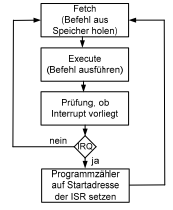
\includegraphics[width=0.45\columnwidth,height=0.21\textheight]{interrupt_fetch}
	\end{wrapfigure}
	\begin{description}[labelindent=0.0cm]
		\item[Prüfung, ob Interrupt vorliegt]~\par
		\begin{enumerate}[leftmargin=0.0cm]
			\item Interrupt unterbricht das aktuell laufende Programm
			\item aktueller Prozessorstatus das laufenden Programms wird am Anfang der Interrupt-Bearbeitung gerettet
			\item Interrupt-Bearbeitungsroutine wird in der Interrupt-Vektor-Tabelle gesucht und ausgeführt
			\item Ende der Bearbeitung: ISR sendet dem Interrupt-Controller Bestätigung
			\item alter Prozessstatus wird hergestellt und es wird an der abgebrochenen Stelle weitergearbeitet
		\end{enumerate}
	\end{description}
	\subsection{Systemdienste und Systemcalls}
	\paragraph{Dienste des Betriebssystems} Anwendungen nutzen die Dienste des Betriebssystems, die über sogenannte Systemcalls aufgerufen werden - Wohldefinierte Einstiegspunkte ins Betriebssystem - Systemcalls werden im Kernelmodus ausgeführt - beim Aufruf wird durch den Prozessor vom Usermodus in den Kernelmodus umgeschaltet
	\section{Prozesse und Threads}
	\subsection{Prozesse und Lebenszyklus von Prozessoren}
	\paragraph{Programm} sind die Dateien und der Programmcode wie sie auf der Festplatte gespeichert sind
	\paragraph{Prozess} Ausführung eines Programms auf einem Prozessor, dynamische Folge von Aktionen verbunden mit entsprechenden Zustandsänderungen, inklusive Daten und Registerinhalten und eigenem Adressraum. Ein Prozess kann folgende Zustände durchlaufen $\rightarrow$ Bereit, Aktiv, Blockiert, Stop, Zombie, Idle, Nicht existent
	\paragraph{Zombie Prozess} ist ein Kindprozess der beendet wurde, aber dessen Elternprozess noch keine Nachricht über dessen "\textit{Ableben}" erhalten hat
	\paragraph{Virtueller Prozessor} jedem Prozess im Multiprogramming wird ein virtueller Prozessor zugeordnet
	\paragraph{Konkurrenz zwischen Prozessen} Prozesse konkurrieren um die Betriebsmittel, laufen abwechselnd einige Millisekunden, werden mit Mitteln des Betriebsystems erzeugt
	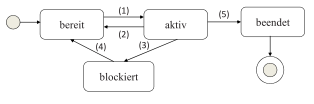
\includegraphics[width=1\columnwidth]{prozesse}
	(1) BS wählt den Prozess aus (Aktivieren)\\
	(2) BS wählt einen anderen Prozess aus (Deaktivieren, Vorrangunterbrechung)\\
	(3) Prozess wird blockiert (z.B. Warten auf Input, Betriebsmittel angefordert)\\
	(4) Blockierungsgrund aufgehoben (Betriebsmittel verfügbar)\\
	(5) Prozessbeendigung oder Fataler Fehler (Terminieren des Prozesses)\\
	\paragraph{Prozesstabelle und PCB} Eintrag in der Prozesstabelle wird als \textit{Process Control Block (PCB)} bezeichnet - wichtige Informationen im PCB: Programmzähler, Prozesszustand, Priorität, Prozess ID, zugeordnete Betriebsmittel, aktuelle Registerinhalte, verbrauchte Prozessorzeit seit Start des Prozesses
	\subsubsection{C Fork()}
	Ein \texttt{fork()} erzeugt einen Kindprozess, der in der nächsten Zeile des Programms beginnt.\\\\
	\begin{allesInCode}
		pid\_d pid; \\
		pid = fork(); \\
		if(pid == 0) \string { \\
		// Kindprozess \\
		printf("Kind-PID: \%u" ,getpid()); \\
		printf("Eltern-PID: \%u" , getpid()); \\
		exit(0); // Prozess Beenden \\
		\string } else \string {\\
		// Elternprozess\\
		\string } \\\\
		if(fork() == 0) \string { \\
		fork(); \\
		\string } \\
		fork(); \\
	\end{allesInCode}
	\subsection{Threads}
	sind leichtgewichtige Prozesse die eine \textit{nebenläufige Ausführungseinheit} innerhalb eines Prozesses darstellen. Alle Threads eines Prozesses teilen sich den gemeinsamen Adressraum dieses Prozesses. Threads haben eigenen Zustandsautomat sowie einen eigenen Programmzähler, einen eigenen Registersatz und einen eigenen Stack. Threads sind genau einem Prozess eindeutig zugeordnet
	\paragraph{Implementierung auf Benutzerebene} Thread - Bibliothek übernimmt das Scheduling und Dispatching für Threads. Der Kernel merkt nicht von Threads
	\paragraph{Implementierung auf Kernelebene} Prozess ist nur noch Verwaltungseinheit für Betriebsmittel. Scheduling-Einheit ist hier der Thread, nicht der Prozess
	\paragraph{Gründe für Threads} Thread-Kontext-Wechsel gehen schneller als Prozess-Kontext-Wechsel, Parallelisierung der Prozessarbeit. Hört auf Netzwerkverbindungswünsche, führt Berechnungen durch, kümmert sich um das User-Interface
	\section{CPU-Scheduling}
	\subsection{Grundlagen}
	\begin{itemize}
		\item CPU-Vergabe in Abhängigkeit der Scheduling-Einheit $\rightarrow$ Prozess- oder Threadbasiert
		\item CPU-Vergabe in Abhängigkeit des Prozesstyps $\rightarrow$ Prozess A CPU-lastig, Prozess B Ein-/Ausgabelastig
	\end{itemize}
	\paragraph{Scheduler} plant die Betriebsmittelzuteilung (teil des Prozessmanagers)
	\paragraph{Dispatcher} zuständig für den Prozesswechsel (teil des Prozessmanagers)
	\paragraph{Zeitscheibenverfahren - (Timesharing} CPU-Zuteilung durch das Betriebssystem. Wenn laufender Prozess auf ein Ereignis wartet oder eine bestimmte Zeit den Prozessor nutzte $\rightarrow$ nächster Prozess. Zeit abhängig vom Quantum, was wiederum abhängig ist von CPU und Betriebssystem
	\subsubsection{Scheduling - Kriterien und Ziele}
	Fairness - jeder Prozess erhält eine garantierte Mindestzuteilung. Effizienz - Möglichst volle Auslastung der CPUs. Antwortzeit - soll möglichst minimiert werden. Verweilzeit (Durchlaufzeit) - Wartezeit von Prozessen soll möglichst klein sein. Durchsatz - Maximierung der Aufträge, die ein Betriebssystem in einem Zeitintervall durchführt.
	\subsection{Scheduling Verfahren}
	\paragraph{Non-preemptive Scheduling} (nicht verdrängend) Prozess wird nicht unterbrochen bis er fertig ist. Ungeeignet für Echtzeitverabeitung oder Dialogbetrieb mit konkurrierenden Benutzern
	\paragraph{Preemptive Scheduling} (verdrängend) rechnende Prozesse können verdrängt werden. Geeignet für konkurrierende Benutzer, aber Zeitscheibentechnik erforderlich
	\subsubsection{Scheduling Algorithmen für Batch-Prozesse}
	\paragraph{First Come First Serve (FCFS)} Nach der Reihenfolge des Eintreffens \textit{(non-preemptive)}
	\paragraph{Shortest Job First (SJF)} Prozess mit kürzester Bedienzeit als erstes \textit{(non-preemptive)}
	\paragraph{Shortest Remaining Time Next (SRTN)} Prozess mit der kürzesten verbleibenden Restzeit im System \textit{(preemptive)}
	\subsubsection{Scheduling Algorithmen für interaktive Prozesse}
	\paragraph{Round Robin (RR)} FCFS in Verbindung mit Zeitscheibe. \textbf{Warteschlange beachten!} Leistung hängt von der Länge der Zeitscheibe ab (kürzeres Quantum=rechenintensive Prozesse, längeres Quantum und/oder höhere Priorität=I/O-Intensive Prozesse). Verhältnis Arbeitszeit/Umlaufzeit darf nicht zu klein sein $\rightarrow$ Durchsatz schlecht \textit{(preemptive)}
	\paragraph{Priority Scheduling (PS)} Prozesse mit höchster Priorität als nächstes. Dynamische und statische Prioritäten und Kombinationen sind möglich \textit{(preemptive oder non-preemptive)}
	\paragraph{Lottery Scheduling} zufällige Vergabe von CPU-Zeit
	\subsubsection{Multi-Level-Scheduling}
	Mehrere Arten von Jobs unterschiedlicher Priorität
	\paragraph{Multi-Level-Feedback-Scheduling} Prozess kann in eine Warteschlange höherer oder niedriger Ordnung wechseln
	\subsubsection{Scheduling in Realtime-Systemen}
	\paragraph{Hard-Realtime-Systeme} müssen unter allen Umständen rechtzeitig reagieren
	\paragraph{Soft-Realtime-Systeme} gelegentliche Verzögerungen erlaubt
	\paragraph{Statische Scheduling-Algorithmen} Scheduling-Entscheidung bereits vor dem Start des Systems bekannt
	\paragraph{Dynamische Scheduling-Algorithmen} Scheduling-Entscheidungen werden zur Laufzeit getroffen
	\subsection{Echtzeit-Scheduling}
	Berechnungen funktional korrekt und rechtzeitig, garantierte Einhaltung von Zeitschranken, Vorhersagbarkeit. Echtzeitsystem besteht aus einer Menge aus Tasks, die quasi parallel arbeiten. Task = Prozess, Thread, etc. $\rightarrow$ wird periodisch ausgeführt und hat eine bestimmte Priorität. Scheduler teilt den Tasks nach einem bestimmten Algorithmus jeweils die CPU zu
	\paragraph{Echtzeitsysteme} Unterstützt harte Echtzeitanforderungen (Garantien), ist auf den Worst-Case hin optimiert, 'Dringende' Prozesse verdrängen weniger wichtige, \textbf{Vorhersagbarkeit} ist wichtig. Sofortige Bearbeitung anstehender Aufträge (Ein-/Ausgabe)
	\paragraph{Universal-Betriebssystem} Unterstützt nur 'weiche' Echtzeitanforderungen (keine Garantien), Optimierung auf die Unterstützung verschiedenster Anwendungsfälle, Reaktionszeit nicht im Vordergrund. Alle Prozesse werden (weitgehend) gleich (fair) behandelt. \textbf{Durchsatz} und Antwortzeitverhalten wichtig, Blockweise Ein-/Ausgabe, Sammlung 'gleicher Aufträge'
	\subsubsection{Statisches Scheduling}
	\paragraph{Rate Monotonic Scheduling (RMS)} Je kürzer die Periode T desto höher die Priorität. Bis zur Deadline D müssen alle Rechenzeiten des jeweiligen Prozesses erledigt sein. \textbf{Vorgehen}: Deadlines/Periodendauer einzeichnen. In jedem Prozess alle seine benötigten Rechenzeiten in jeder Periode einzeichnen, dies nach Priorität machen. Die Priorität wird in jedem Schritt neu überprüft. Dabei gegebenenfalls den Prozess unterbrechen und mit dem Prozess der höheren Priorität weitermachen
	\paragraph{Major cycle} (auch Hyper Period) nach einem major ciycle wiederholt sich das Verhalten des Systems
	\paragraph{Critical Instant (CI)} alle Tasks wollen zur selben Zeit starten $\rightarrow$ stellt das \textbf{worst case} szenario dar. Wird dieser ohne Deadline-Überschreitung überstanden, so werden immer alle Deadlines eingehalten
	\paragraph{Response-Time Analyse (RTA)} maximale Antwortzeit $R_i$ einer Task $i$ $\rightarrow$ $R_i =$ eigene Ausführungszeit $C_i +$ 'Störungen' - System ist echtzeitfähig, wenn für alle Tasks $i$ die Antwortzeit der Deadline ist $\rightarrow$ $R_i D_i$
	\subsubsection{Dynamisches Scheduling}
	zur Laufzeit wird entschieden, welche Task die höchste Priorität bekommt
	\paragraph{Earliest-Deadline First (EDF)} Task mit der nächsten absoluten Deadline hat die höchste Priorität und die absolute Deadline ist abhängig vom Zeitpunkt- \textbf{Vorteil} ist hohe Prozessorauslastung, einfacher Schedulability Test. \textbf{Nachteil} ist, für den Scheduler entsteht ein erheblich größerer und im Aufwand schwankender Overhead als bei statischen Verfahren
	\subsubsection{Beispiel Wartezeiten}
	\begin{tabularx}{\columnwidth}{|l|X|X|X|X|X|c|c|}
		\cline{1-8}
		Job & A & B & C & D & E & $W_{all} = \sum \limits_{i=1}^n W_i$ & $W_{avg} = \frac{1}{n}W_{all}$ \\
		\cline{1-8}
		Ablaufzeit & 8 & 27 & 1 & 5 & 10 & & \\
		\cline{1-8}
		\multicolumn{8}{|l|}{FCFS} \\
		\cline{1-8}
		Job & A & B & C & D & E & & \\
		\cline{1-8}
		Wartezeit & 0 & 8 & 35 & 40 & 41 & 124 & 24,8\\
		\cline{1-8}
		\multicolumn{8}{|l|}{SJF} \\
		\cline{1-8}
		Job & C & D & A & E & B & &\\
		\cline{1-8}
		Wartezeit & 0 & 1 & 6 & 14 & 24 & 45 & 9\\
		\cline{1-8}
		\multicolumn{8}{|l|}{RR mit 2ms Zeitscheibe (Quantum)} \\
		\cline{1-8}
		Job & \multicolumn{7}{c|}{A-B-D-\textbf{C}-E-A-B-D-E-A-B-\textbf{D}-E-\textbf{A}-B-E-B-\textbf{E}-B-...-\textbf{B}} \\
		\cline{1-8}
		Job & A & B & D & C & E & $W_{all} = \sum \limits_{i=1}^n W_i$ & $W_{avg} = \frac{1}{n}W_{all}$ \\
		\cline{1-8}
		Wartezeit & 18 & 24 & 17 & 6 & 24 & 89 & 17,8\\
		\cline{1-8}
	\end{tabularx}
	\section{Synchronisation und Kommunikation}
	\subsection{Grundlegendes zur Synchronisation}
	\subsubsection{Nebenläufigkeit, atomare Aktionen und Race Conditions}
	\paragraph{Nebenläufigkeit} parallele bzw. quasi-parallele Ausführung von Befehlen auf einer oder mehreren CPUs. Prozesse bzw. Threads werden in Multiprogramming-Systemen nebenläufig ausgeführt - Programmierer kann die Ablaufreihenfolge nicht beeinflussen
	\paragraph{Race Condition} Zwei oder mehrere Prozesse/Threads benutzen ein gemeinsames Betriebsmittel. Das Endergebnis ist von der zeitlichen Reihenfolge abhängig $\rightarrow$ Inkonsistenzen
	\paragraph{Atomare Aktion} Codebereiche des Betriebssystem (oder Anwendung), die in einem Stück ausgeführt werden müssen und nicht unterbrochen werden dürfen. Prozesse, die atomare Aktionen durchführen müssen exklusiv Betriebsmittel zugeteilt werden und dürfen dem Prozess nicht entzogen werden - Unterbrechung durch eine Scheduling-Entscheidung des Betriebssystem jederzeit möglich
	\paragraph{Beispiel} verkettete Listen werden vom Betriebssystem verwaltet $\rightarrow$ von mehreren Prozessen zugreifbar - Operation besteht aus zwei Kommandos - Prozess möchte ein neues Objekt an die Liste hängen, genau wie ein anderer Proess und wird unterbrochen - Prozess B, welcher die selben Variablen wir Prozess  A verwendet, könnte ein Problem verursachen
	\paragraph{Lost-Update-Problem} Inkonsistenzen bei gemeinsam genutztem Zähler, der von zwei Prozessen verändert wird
	\subsubsection{Kritische Abschnitte und wechselseitiger Ausschluss}
	\paragraph{kritische Abschnitte} sind Programmteile, die nicht unterbrochen werden dürfen. Codeabschnitt, der zu einer Zeit nur durch einen Prozess durchlaufen wird - nebenläufige Prozesse dürfen nicht dazu treten - Prozess bzw. Thread, der den kritischen Abschnitt belegt, darf durch eine Scheduling-Entscheidung des Betriebssystems nicht beeinflusst werden
	\paragraph{wechselseitiger Ausschluss} schützt einen kritischen Abschnitt - Prozesse, die einen kritischen Abschnitt ausführen wollen, müssen warten bis dieser frei ist - Illusion einer atomaren Anweisungsfolge wird erschaffen - nur Illusion, da ein nebenläufiger Prozess zwischendurch die CPU erhalten kann
	\paragraph{Busy Waiting} Warten und ständige Abfragen eines Sperrkennzeichens am Eingang des kritischen Abschnitts, der freigegeben werden muss\\
	Effizienter: Prozess, der einen kritischen Abschnitt belegen will, schlafen legen und ihn wieder wecken wenn der Abschnitt frei ist. Zu einer Zeit ist immer nur ein Prozess im kritischen Abschnitt
	\paragraph{Kriterien nach Dijkstra} \textit{Mutual Exclusion}: Zwei oder mehr Prozesse dürfen sich nicht gleichzeitig im gleichen kritischen Abschnitt befinden.\\ Es dürfen keine Annahmen über die Abarbeitungsgeschwindigkeit und die Anzahl der Prozesse bzw. Prozessoren gemacht werden.\\ Kein Prozess außerhalb eines kritischen Abschnitts darf einen anderen nebenläufigen Prozess
	\textbf{blockieren}. \\\textit{Fairness Condition}: Jeder Prozess, der am Eingang eines kritischen Abschnitts wartet, muss ihn irgendwann betreten dürfen \textbf{()kein ewiges Warten)}
	\subsubsection{Eigenschaften nebenläufiger Prozesse}
	\paragraph{Blockieren} Ein Prozess belegt Betriebsmittel, welche ein anderer Prozess benötigt
	\paragraph{Verhungern} Prozess erhält trotz Rechenbereitschaft keine CPU-Zeit zugeteilt
	\paragraph{Verklemmung} zwei oder mehrere Prozesse halten jeder für sich ein oder mehrere Betriebsmittel belegt und versuchen ein weiteres zu belegen, das aber von dem anderen Prozess belegt wird $\rightarrow$ kann zu \textbf{Dead Lock} führen
	\paragraph{Dead Lock} Verklemmung, es liegt eine Abhängigkeit vor. Kein Prozess gibt seine Betriebsmittel frei, und alle Prozesse warten daher ewig. Bedingungen: \textbf{Mutual Exclusion} für die benötigten Betriebsmittel\\ Prozesse \textit{belegen} Betriebsmittel und \textbf{fordern weitere} an\\ \textbf{Kein Entzug} eines Betriebsmittels \textbf{möglich}\\ Zwei oder mehrere Prozesse \textbf{warten} in einer Warteschleife auf \textbf{weitere Betriebsmittel}
	\paragraph{Sicherheit} es befinden sich nie zwei Prozesse in einem kritischen Abschnitt und es kommen nie Verklemmungen vor
	\paragraph{Lebendigkeit} ein Prozess kann nach einer evtl. Wartezeit in einen kritischen Abschnitt eintreten (wenn alle gewünschten Zustände eintreten)
	\subsection{Synchronisationskonzepte}
	\subsubsection{Sperren}
	Eine einfache Lösung zur Realisierung von kritischen Abschnitten ist busy waiting (aktives Warten). Ein Prozess testet eine sog. Synchronisationsvariable solange, bis die Variable einen Wert hat, der den Zutritt erlaubt. Dieses Polling ist oft unwirtschaftlich, da es eine Verschwendung der CPU-Zeit bedeutet, aber: Spinlocks in Betriebssystemen sind oft anzutreffen (bei sehr kurzen Wartezeiten bei Multiprozessoren gut). Meist ist es besser, einen Prozess 'schlafen' zu legen und erst wieder wecken, wenn er in den kritischen Abschnitt darf.
	\paragraph{Hardwareunterstützung durch Maschinenbefehle} Problem: Zwei CPUs führen einen \textit{TSL-Befehl} (Test and Set Lock) aus und die Teiloperationen überlappen sich. Ausführung eines TSL-Befehls in einem Speicherzyklus erledigt $\rightarrow$ funktioniert bei Multiprocessing. Operanden des TSL $\rightarrow$ TSL R1, LOCK $\rightarrow$ LOCK in R1 einlesen und LOCK auf 1 setzen
	\subsubsection{Semaphore}
	Dijkstra (1965) führte das Konzept der Semaphore zur Lösung des Mutual Exclusion Problems ein. Semaphore selber müssen unterbrechbar sein, da ein Unterbrechen dieser Operationen zu Inkonsistenzen führen kann. Zwei elementare Operationen:
	\paragraph{P()} P-Operation, auch \textbf{Down}-Operation genannt. Aufruf bei Eintritt in den kritischen Abschnitt, Operation auf Semaphor. Aufrufender Prozess wird in den Wartezustand versetzt, wenn sich ein anderer Prozess im kritischen Abschnitt befindet $\rightarrow$ Warteschlange
	\paragraph{V()} V-Operation, auch \textbf{Up}-Operation genannt. Aufruf bei Verlassen des kritischen Abschnitts, evtl. wird einer der wartenden Prozesse aktiviert und darf den kritischen Abschnitt betreten\\\\
	Nutzung des Semaphors könnte so aussehen:\\
	\begin{allesInCode}
		Down(); // kritischer Abschnitt besetzt? \\
		c=counter.read(); // kritischer Abschnitt \\
		c++; \\
		counter.write(c); \\
		Up(); // Verlassen des kritischen Abschnitts \\
		// Aufwecken eines wartenden Prozesses \\
	\end{allesInCode}
	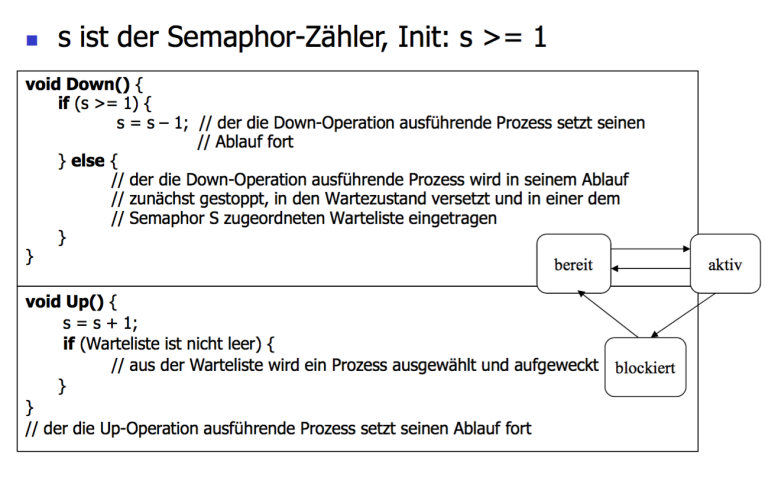
\includegraphics[width=0.9\columnwidth]{semaphor}
	\paragraph{Mutex} Wenn man auf den Zähler im Semaphor verzichten kann, kann eine einfachere Form angewendet werden. Ein Mutex ist leicht und effizient zu implementieren. Ein Mutex ist eine Variable, die nur zwei Zustände haben kann. \textit{locked} und \textit{unlocked}. Man braucht also nur 1 Bit zur Implementierung
	\subsection{Synchronisationsprobleme}
	\subsubsection{Erzeuger-Verbraucher-Problem}
	Ein ohder mehrere Erzeugerprozesse (producer) produzieren, ein oder mehrere Verbraucherprozesse (consumer) konsumieren. Flusskontrolle erforderlich. Erzeuger legt sich schlafen, wenn Puffer voll ist und wird vom Verbraucher aufgeweckt, wenn wieder Platz ist. Verbraucher legt sich schlafen, wenn Puffer leer ist und wird vom Erzeuger wieder aufgeweckt, wenn wieder was drinnen ist\\
	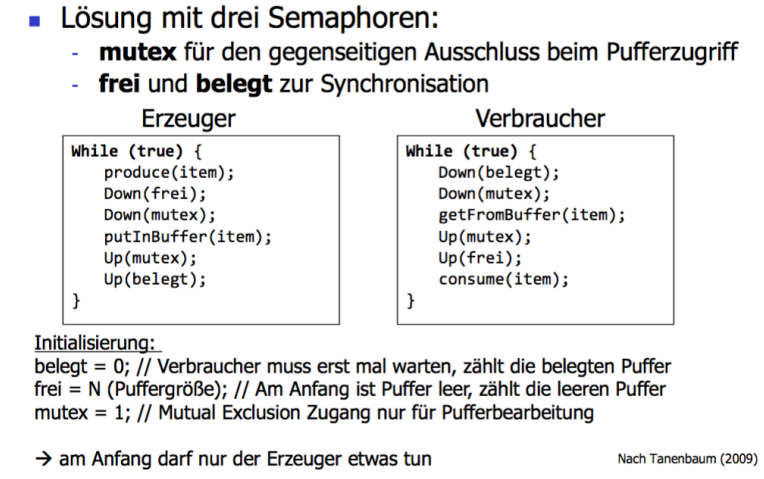
\includegraphics[width=0.9\columnwidth]{erzeuger-verbraucher}
	\subsection{Synchronisation in Programmiersprachen}
	\subsubsection{Monitore}
	Abstrakter Datentyp, Erzeugung und Anordnung der Semaphor-Operationen dem Compiler überlassen. Menge von Prozeduren und Datenstrukturen - werden als Betriebsmittel betrachtet $\rightarrow$ für mehrere Prozesse zugänglich, kann nur von einem Prozess zu einer Zeit genutzt werden. Zusammengefasst: ein Objekt, das den Zugriff auf gemeinsame Daten über kritische Bereiche in Zugriffsmethoden realisiert, gemeinsam benutzte Daten werden durch Synchronisationsvariable geschützt\\
	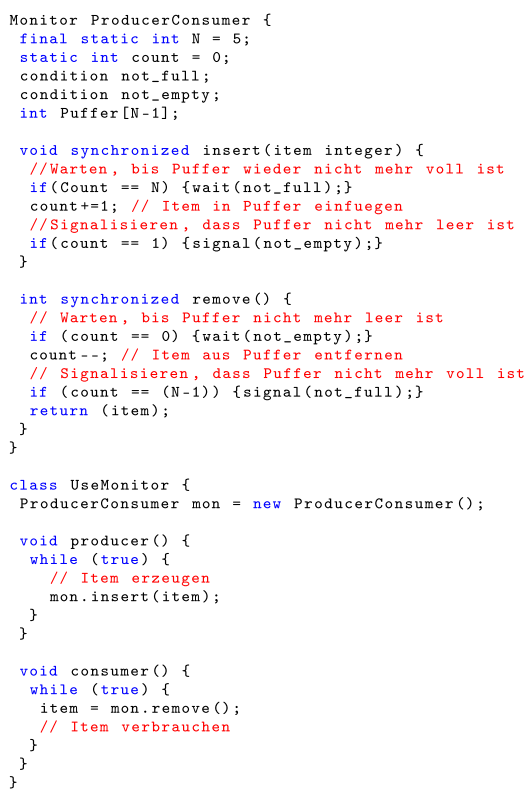
\includegraphics[width=0.65\columnwidth]{monitor}
	\paragraph{synchronized} ermöglicht eine Zugriffsrealisierung. Methoden und Codeblöcke, die mit \textit{synchronized} gekennzeichnet wurden, bilden gemeinsam einen kritischen Abschnitt. Bei Eintritt eines Threads in einem mit \textit{synchronized} gekennzeichneten Bereich werden alle kritischen Bereiche des Objekts gesperrt
	\subsubsection{Methoden zur expliziten Synchronisierung}
	\texttt{wait()}: Thread wartet auf ein \textit{notify} eines anderen Threads\\
	\texttt{notify()}: weckt mindestens einen wartenden Thread auf \\
	\texttt{notifyAll()}: alle Threads, die auf das gleiche Objekt warten, werden geweckt\\
	\texttt{wait()} und \texttt{notify()} dürfen nur innerhalb eines mit \textit{synchronized} geschützten Abschnitt aufgerufen werden
	\subsubsection{C\# Monitore}
	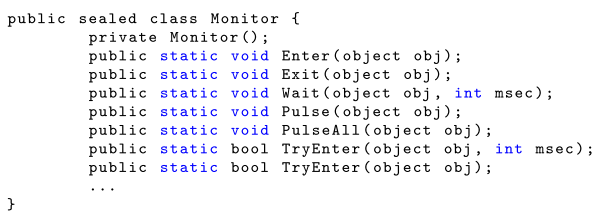
\includegraphics[width=0.65\columnwidth]{monitor_csharp}
	\subsection{Behandlung von Deadlocks}
	Allgemein gilt, Deadlocks sind unmöglich falls $r = 1 + (p \cdot (m-1))$ wobei $p =$ Prozesse, $r = $ Ressourcen und $m =$ maximal benötigte Ressourcen pro Prozess ist
	\subsubsection{Ignorieren}
	Nur sinnvoll, wenn Deadlocks selten auftreten oder Kosten der Vermeidung sehr hoch sind. Unakzeptabel in Echtzeitsystemen oder Kosten eines Deadlocks sehr hoch sind
	\subsubsection{Erkennen und beheben}
	Deadlocks sind grundsätzlich zugelassen, werden zur Laufzeit erkannt. Deadlockerkennung z.B. über Betriebsmittelbelegungsgraphen. Beheben durch $\rightarrow$ \textbf{Unterbrechung} (Entziehung der Ressource eines Prozesses, nicht immer möglich), \textbf{Rollbacks} (Checkpoints regelmäßig setzen), \textbf{Prozessabbruch}, \textbf{Transaktionsabbruch}
	\subsubsection{Dynamisch Verhindern}
	Verhindernd, dass die Ressourcenspur in den gefährlichen Bereich (\textbf{unsicheren Zusatnd}) gerät. Die Ressourcen vorsichtig zuteilen
	\paragraph{Sichere und unsichere Zustände} Ein Zustand heißt sicher, wenn es mindestens eine Scheduling-Reihenfolge gibt, die nicht zum \textit{Deadlock} führt\\
	Beispiel: Insgesamt sind 10 Instanzen einer Ressource verfügbar\\
	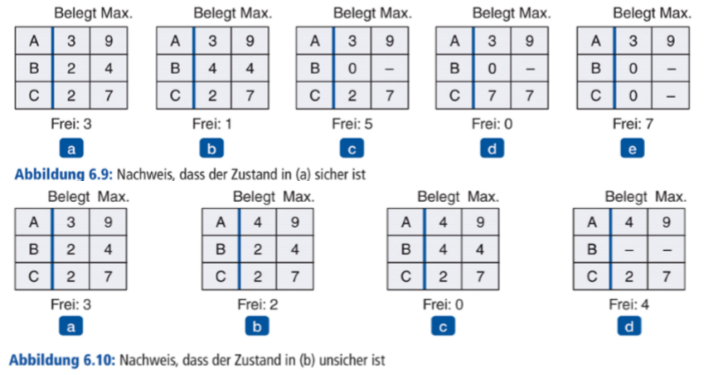
\includegraphics[width=0.98\columnwidth]{zustand}
	\paragraph{Banker-Algorithmus} Der Banker räumt ein 'Kreditlimit' in und achtet darauf, dass sein verleihbares Kapital beim Ausleihen nicht überschritten wird $\rightarrow$ Ziel: unsichere Zustände verhinder\\
	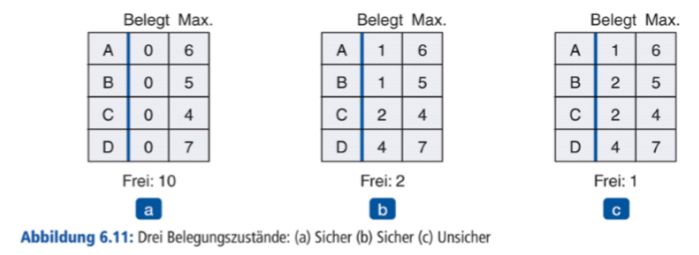
\includegraphics[width=0.9\columnwidth]{banker}
	Nachteile: Bestimmung des Betriebsmittels-Bedarfs a-priori meist nicht möglich. Außerdem braucht der Algorithmus viel Rechenzeit und Speicherplatz. Das Verfahren garantiert zwar das jeder Prozess in endlicher Zeit seine Betriebsmittel bekommt, liefert aber keine Zeitschranken
	\subsubsection{Vermeiden}
	\paragraph{Mutual exclusion} unvermeidbar, manchmal ist \textbf{Spooling} (Nur ein Prozess kann zugreifen und Ressource wird virtualisiert) möglich
	\paragraph{Hold-and-Wait} Prozess muss alle benötigten Ressourcen auf einmal anfordern $\rightarrow$ danach muss er nicht mehr auf die Ressource warten. Probleme: Ressourcenbedarf nicht immer zu Beginn bekannt, Ressourcen sind länger wie nötig ist belegt. \textit{Variante}: Bevor eine zusätzliche Ressource angefordert wird, müssen alle bisher belegten zuerst freigegeben werden
	\paragraph{No preemption} Ist keine Option, z.B. Drucker $\rightarrow$ riesige Wartezeit
	\paragraph{Circular Wait} Ressourcen aufsteigend nummeriert. Ressourcen nur in aufsteigender Reihenfolge anforderbar $\rightarrow$ Belegungsgraph bleibt immer zyklenfrei. Probleme: Alle Prozesse müssen sich an die Vereinbarung halten, Ändert sich die Nummerierung müssen alle Prozesse angepasst werden
	\subsubsection{Echtzeitsysteme}
	Menge von periodischen Tasks mit festen Prioritäten. Vorhersagbar, d.h. Laufzeit und Ressourcenbedarf jeder Task bekannt
	\paragraph{Priority Ceiling Protokoll} Jede Ressource bekommt eine Ceiling Priority (maximale Priorität des Tasks die sie nutzen wollen). Belegt ein Task eine Ressource, bekommt sie die Ceiling Priority dieser Ressource $\rightarrow$ Unterlaufen der \textit{Circular Wait} Bedingung
	\section{Kommunikation}
	Austausch von Informationen zwischen (Menschen), (Mensch und Maschine $\rightarrow$ Rechnersystem), (Maschinen $\rightarrow$ Prozesse/Threads)
	\paragraph{Verbindungsorientiert} Vor dem Datenaustausch wird eine logische Verbindung aufgebaut und danach wieder abgebaut. Kommunikationspartner kennen Verbindungspartner
	\paragraph{Verbindungslos} Daten ohne Verbindungsmanagement vom Sender zum Empfänger übertragen. Senderadresse in der Nachricht mit übertragen
	\paragraph{Speicherbasiert} Daten werden in einem gemeinsamen Speicher ausgetauscht oder 'geshared'
	\paragraph{Nachrichtenbasiert} Zwischen Prozessen/Threads werden Nachrichten ausgetauscht $\rightarrow$ einheitliches Protokoll
	\paragraph{synchrone Kommunikation} ist blockierend
	\paragraph{asynchrone Kommunikation} ist nicht blockierend
	\paragraph{Halbduplex} Nur einer der Partner sendet zu einer Zeit
	\paragraph{Vollduplex} beide Partner können unabhängig voneinander senden
	\paragraph{Varianten} \textbf{der Empfängeradressierung}\\
	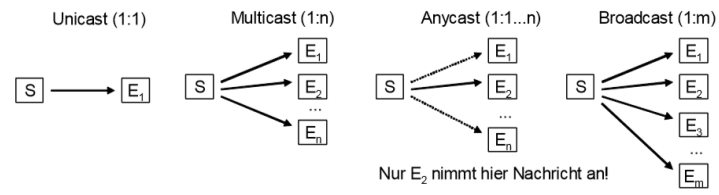
\includegraphics[width=0.8\columnwidth]{adressierung}
	\paragraph{Pipes} Spezieller \textit{unidirektionaler} Mechanismus - bidirektioale Kommunikation durch Nutzung mehrerer Pipes - bidirektionale Kommunikation kann sowohl halb- als auch vollduplex betrieben werden. Standardeingabe eines Prozesses kann mit der Standardeingabe eines weiteren Prozesses verbunden werden
	\paragraph{Pipes -} \textbf{Programmierung}
	\begin{itemize}
		\item Erzeugen - Unix \texttt{pipe()} oder \texttt{popen()}
		\item Schließen - Unix \texttt{close()} oder \texttt{pclose()}
		\item Elternprozess erzeugt Pipe und vererbt sie an den Kindprozess - blockierend und nicht blockierend einsetzbar (Pipe voll $\rightarrow$ Sendermodus blockiert, Pipe leer $\rightarrow$ Leseprozess blockiert)
	\end{itemize}
	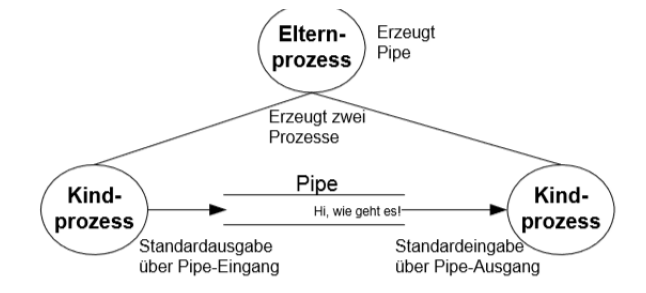
\includegraphics[width=0.65\columnwidth]{pipe}
	\paragraph{Verteilte Kommunikation zwischen Prozesse/Threads} Betriebssystem stellt Kommunikationssystem bereit, Netzzugang erforderlich
	\section{Speicherverwaltung}
	Reihenfolge, nach Zugriffsgeschwindigkeit: Register $\rightarrow$ Cache $\rightarrow$ Hauptspeicher $\rightarrow$ Magnetische Platten oder SSD $\rightarrow$ Magnetische Bandlaufwerke
	\begin{description}[labelindent=0.0cm]
		\item[Lokalitätsprinzip]~\par
		\begin{itemize}[leftmargin=0.0cm]
			\item \textbf{Zeitlich}: Daten/Code-Bereiche, die gerade genutzt werden, sollten für die nächste Nutzung bereitgehalten werden
			\item \textbf{Örtlich}: Benachbarte Daten beim Zugriff auch gleich in schnelleren Speicher laden
			\item \textbf{Working Set}: Lokaler Code- bzw. Datenabschnitt, in dem ein Prozess vorwiegend arbeitet
		\end{itemize}
	\end{description}
	\paragraph{Adressraumbelegung} Durch den Adressraumbelegungsplan bestimmt - Festlegung im Betriebssystem - Ausrichtung auf Maschinenwörter $\rightarrow$ optimaler Zugriff - Compiler/Interpreter organisiert Bereich für Anwendungsprogramme
	\paragraph{Cache} Schneller Speicher mit kleiner Kapazität, wo Daten ein- und ausgelagert werden $\rightarrow$ möglichst viele Daten im Cache finden. \textbf{Cache hit} oder \textbf{Cache miss} $\rightarrow$ Rückgriff auf langsamere Ebene - Ziel auf allen Ebenen: Möglichst hohe Trefferrate. \textbf{Cache-Prinzip}: Je häufiger auf Daten zugegriffen wird, desto schneller sollte der Zugriff sein. \textbf{Einlagern}: Ganzer Datenblock aus Umgebung wird nach einem Cache miss geladen $\rightarrow$ Lokalitätsprinzip - Cache ist immer komplett gefüllt
	\paragraph{least recently uses (LRU)} Austausch des am längsten nicht mehr referierten Cache-Block. HW-Alterungszähler für jeden Cache-Block, bei Zugriff wird dieser auf 0 gesetzt, alle anderen um 1 erhöht. Block mit dem höchsten Zählerstand wird ausgelagert
	\paragraph{least frequently accesses (LFA)} Austausch des am wenigsten benutzten Cache-Blocks. HW-Referenzzähler auf den Cache-Block um 1 erhöht und durch das Betriebssystem nach einem Zeitintervall bzw. nach Austausch auf 0 gesetzt wird
	\paragraph{least recently loaded (LRL)} Austausch des am längsten geladenen Cache-Blocks. Festhalten und späterer Vergleich des Ladezeitpunktes $\rightarrow$ FIFO-Verfahren
	\paragraph{Zufallsauswahl} Auszutauschender Block wird zufällig gewählt $\rightarrow$ geringer Aufwand
	\subsection{Schreiboperationen}
	\paragraph{Durchschreiben (write through)} Jede Schreiboperation auf einem Cache-Block wird sofort auch auf der unterliegenden Speicherebene durchgeführt
	\paragraph{Zurückschreiben (write back)} Schreiboperationen wirken zunächst nur auf den Cache-Block. Erst beim Austausch des Blocks werden Daten auch an der langsameren Ebene geändert
	\paragraph{Schreiben auf Anforderung (write on demand)} Schreiboperationen an der langsameren Ebene werden nur auf besondere Anforderung durchgeführt (bei Prozesswechsel)
	\paragraph{Trefferrate} hängt ab von der Cache-Größe, von der Ersetzungsstrategie, von der Programm- und Datenorganisation
	\subsection{Mechanismen der Speicherverwaltung}
	\paragraph{Monoprogramming} einfachste Form der Speicherverwaltung $\rightarrow$ nur ein Programm läuft zu einer Zeit
	\paragraph{Mit festen Partitionen} Aufteilung eines Speichers in feste Teile (Partitionen) - Multiprogramming un Verbesserung der CPU-Auslastung möglich - Job wird in eine Queue eingetragen
	\subsubsection{Speicherverwaltung bei Multiprogramming mit Swapping}
	\paragraph{Grundgedanke: Timesharing} Es passen nicht immer alle Prozesse in den Hauptspeicher - Prozess wird im Gesamte geladen - Prozess wird irgendwann auf einen Sekundärspeicher ausgelagert - Löcher können durch Kombination benachbarter Speicherbereiche eliminiert werden (aufwändig)
	\paragraph{Hauptunterschied zu festen Partitionen} Anzahl, Speicherplatz und Größe des für einen Prozess verwendeten Speicherbereichs variieren dynamisch - Prozess wird da geladen, wo Platz ist
	\subsection{Grundprinzipien des virtuellen Speichers}
	Speichergröße eines Programms darf den vorhandenen physikalischen Hauptspeicher überschreiten - Prozess kann ablaufen, wenn er nur teilweise im Hauptspeicher ist - Programmierer soll sich am besten nur mit einem linearen Adressraum befassen - Betriebssystem hält die gerade benutzten Teile im Hauptspeicher und den Rest auf der Festplatte
	\paragraph{Virtueller Adressraum} Wird vom Prozess gesehen, ist in \textit{Seiten} aufgeteilt
	\paragraph{Realer Adrssraum} RAM, normalerweise kleiner als virtueller Adressraum, ist in \textit{Seitenrahmen} aufgeteilt
	\paragraph{Seite} Teile eines virtuellen Adressraums. Mehrere Speicherseiten bilden Speicherabbild eines Prozesses - nur die benötigten Speicherseiten müssen im Arbeitsspeicher geladen sein, während der Prozess läuft - Größe meist gering, Anzahl beliebig groß. Kleine Seitengröße $\rightarrow$ mehr Seitenfehler, Seitentabelle wird größer
	\paragraph{Seitenrahmen} Teile eines realen Adressraums. \textit{Seiten} und \textit{Seitenrahmen} müssen zwingend die gleiche Größe haben
	\subsubsection{Strategien zur Verwaltung von virtuellem Speicher}
	\paragraph{Paging} Umlagerung zwischen Hauptspeicher und Festplatte. Jeder Prozess darf alle Adressen verwenden, welche die HW-Architektur des Rechners vorgibt - bei Systemen mit 32-Bit-Adressen kann jeder Prozess einen Adressraum von 4GiB verwenden
	\paragraph{Memory Management Unit (MMU)} CPU sendet virtuelle Adressen an die MMU, welche daraus die reale Adresse ermittelt und sie an den Hauptspeicher weiterleitet
	\paragraph{Adressumsetzung} Virtuelle Adresse ist in virtueller \textit{Seitennummer} und einem \textit{Offset} geteilt - virtuelle Seitennummer ist ein Index auf die \textit{Seitentabelle} - im Eintrag steht die Rahmen-Nummer, falls die Seite einem Rahmen zugeordnet ist. Befindet sich eine angesprochene Adresse nicht im Hauptspeicher $\rightarrow$ MMU verursacht bei der MMU einen \textbf{Trap}\\ \textbf{Berechnung}: Teile \textbf{Virtuelle Adresse} durch \textbf{Seitengröße} $\rightarrow$ \textbf{Ganzzahliger Anteil} gibt die Zeile im virtuellen Adressraum an. Diese Zeile gibt den Rahmen im realen Adressraum an. An den dort angegeben wert muss der \textbf{Offset} (Rest der Divisionsoperation) addiert werden $\rightarrow$ physische Adresse\\\\
	Mapping muss schnell sein - in großen Adressräumen sind sehr große Seitentabellen möglich (32 Bit Adressraum $\rightarrow$ 1 Mio. Einträge, Seitengröße von 4 KiB)(Bei 4 Byte pro Eintrag $\rightarrow$ 4MiB Hauptspeicher notwendig)
	\paragraph{Mehrstufige Adressumsetzung} Spart Speicherplatz da Seitentabellen nicht komplett im Speicher gehalten werden müssen. Virtuelle Adresse enthält Index Bits für jede Stufe der Seitentabelle. Beispiel: 32 Bit Virtuelle Adresse, zwei Stufig mit je 1024 Plätzen $\rightarrow$ 10 Bit für Index 1, 10 Bit für Index 2 und 12 Bit für Offset\\
	\textbf{Berechnung} der Seiten im Adressraum: 2\^{}(Summe \textbf{aller} Indexbits der virtuellen Adresse). Beispiel oben wäre 2\^{}20 = 1.048.576
	\paragraph{Seitentabelle} Jeder Prozess hat seine eigene Seitentabelle. Der Virtuelle Adressraum zeigt auf einen Index in der Seitentabelle. Über den Index findet man die Position des gewünschten Seitenrahmen
	\paragraph{Page Fault (Seitenfehler)} Wenn eine benötigte Seite nicht im realen Speicher liegt, wird von der \textit{MMU} ein Interrupt der sogenannte Page Fault erzeugt, der dafür sorgt das die benötigte Seite in den Hauptspeicher geladen wird.
	\subsection{Optimierung der virtuellen Speichertechnik}
	\paragraph{Virtuelle Adressierung aufwändig, da...} viele, umfangreiche Tabellen benötigt werden - Teil der Festplatte wird als Paging-Area verwendet - laufend muss untersucht werden, ob Seiten im Hauptspeicher bleiben oder auf die Festplatte auszulagern sind
	\paragraph{Optimierung durch Adressumsetzpuffer...} größere Seiten (64-Bit-Prozessoren)
	\paragraph{Translation Lookaside Buffer (TLB)} Adressumsetzpuffer ist ein schnelles Speicherabbild - Zuordnung von virtuellen auf reale Adressen für die aktuell am \textit{häufigsten} benötigten Adressen - bei der Adressumsetzung wird zuerst in dem TLB geschaut $\rightarrow$ \textbf{Hit}: Kein Zugriff auf Seitentabelle nötig - Einsparung von Hauptspeicherzugriffen. Dadurch ist eine Beträchtliche Leistungsoptimierung möglich. Der TLB ist Bestandteil der MMU. Ein TLB-Eintrag enthält: Virtuelle Seitennummer, Verweis auf den Seitenrahmen im Hauptspeicher, Tag zur Adressraum-Identifikation $\rightarrow$ Tagged TLB
	\subsubsection{Optimierung durch invertierte Seitentabellen}
	angelegte Tabelle, in der man reale Adressen auf virtuelle abbildet - ein Eintrag pro Frame in einer invertierten Seitentabelle - \textbf{Vorteil}: weniger Tabelleneinträge $\rightarrow$ nur noch so viele wie Seitenrahmen im Hauptspeicher zu Verfügung stehen - \textbf{Nachteil}: In der Seitentabelle ist keine Ordnung nach virtuellen Adressen $\rightarrow$ Suche aufwändiger
	\paragraph{Virtuelle Speichertechnik} \textbf{Vorteile}: Prozesse müssen nicht komplett speicherresident sein - lineare Speicheradressierung - beim Prozesswechsel behält ein Prozess seine hauptspeicherresidenten Seiten - Anwendungsprogramme können vollen virtuellen Adressraum nutzen
	\subsection{Seitenersetzung und Verdrängung}
	\subsubsection{Belady} Es werden die Seiten zur Verdrängung ausgewählt, die \textbf{am spätesten in der Zukunft} benutzt werden $\rightarrow$ zukünftige Seitenzugriffe müssen bekannt sein $\rightarrow$ \textbf{kaum realisierbar, aber sinnvoll als Referenz}
	\subsubsection{Seitenersetzungsalgorithmen}
	\paragraph{Demand-Paging} Ersetzung einer Seite nur bei Page Fault
	\paragraph{First-In, First-Out (FIFO)} Die älteste Seite wird ersetzt, leicht zu implementieren. \textbf{Nachteil}: Möglicherweise werden wichtige Seiten entfernt
	\paragraph{Not-Recently-Used (NRU)} Seiten, die \textbf{in letzter Zeit nicht genutzt wurden}, sind Kandidaten für Verdrängung. Seiten haben \textbf{R/M-Bits} (read, modiefied). Modifizierte Seiten sind besser gestellt. Entfernung nach folgender Reihenfolge
	\begin{tabularx}{\columnwidth}{|l|l|l|X|}
		\cline{1-4}
		\multicolumn{4}{|c|}{4 Klassen "Opfersuche" in dieser Reihenfolge} \\
		\cline{1-4}
		Nr & R-Bit & M-Bit & Beschreibung\\
		\cline{1-4}
		1 & 0 & 0 & Seiten werden als erstes ausgelagert \\
		\cline{1-4}
		2 & 0 & 1 & Verändert im vorhergehenden Intervall \\
		\cline{1-4}
		3 & 1 & 0 & Nur lesender Zugriff im aktuellen Intervall \\
		\cline{1-4}
		4 & 1 & 1 & Seiten werden als letztes ausgelagert \\
		\cline{1-4}
	\end{tabularx}
	\paragraph{Second Chance} Ist eine Verbesserung von \textbf{FIFO}. Nutzt zusätzlich das \textbf{R-Bit} $\rightarrow$ Aging. Ist die älteste Seite schon benutzt, wird sie nicht ausgelagert, sondern an das Ende der Liste gehängt und das \textbf{R-Bit} gelöscht (auf 0 gesetzt). Wurden alle Seiten in einem Intervall referenziert $\rightarrow$ wie FIFO-Algorithmus
	\paragraph{Clock-Page} Verbesserung von \textit{Second Chance}. Statt \textit{FIFO} eine \textbf{zyklisch verkettete Liste} (wie eine Uhr). "Uhrzeiger" verweist auf Kandidaten und wandert durch die Liste. Falls \textbf{R = 1 $\rightarrow$ R = 0} setzen und weiter schalten bis eine Seite mit \textbf{R = 0} gefunden ist
	\paragraph{Least Recently Used (LRU)} Ersetzt die Seiten die Zeitlich am weitesten zurück liegen. Liefert gute Ergebnisse, aber \textbf{aufwändig}. \textbf{Zeitmessung} notwendig
	\paragraph{Not Frequently Used (NFU)} Gute Annäherung an \textit{LRU}. Ersetzt Seiten, die in \textbf{einem Zeitintervall selten genutzt} wurden. Seitentabelle erhält einen Eintrag mit \textbf{Zugriffszähler} (initialisiert mit 0). Bei Benutzung wird \textbf{Zähler} um 1 erhöht. Bei \textit{Page Fault} $\rightarrow$ Ersetze Seite mit \textbf{kleinstem Zähler}. Problem ist, alte, häufig zugegriffene Seiten die nicht mehr verwendet werden, werden nicht ausgelagert $\rightarrow$ Alterung berücksichtigen, \textbf{Aging}
	\paragraph{Aging Algorithmen (1)} NxN \textbf{Bitmap}. Bei Zugriff auf Seite k $\rightarrow$ 1. Setze alle Bits in \textbf{Zeile k} auf 1\\ 2. Setze alle Bits in \textbf{Spalte k} auf 0
	\paragraph{Aging Algorithmen (2)} Ein \textbf{Zähler pro Seite}. Periodisch in festen Zeitintervallen werden alle Zähler um \textbf{ein Bit nach rechts geschiftet} und \textbf{R-Bit} zum linken (höchstwärtigen) Bit addieren\\
	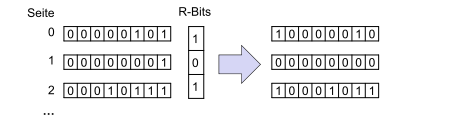
\includegraphics[width=1.05\columnwidth]{aging}
	\paragraph{Working Set} Aktuell benötigte Seitenmenge = \textbf{Working Set}. Ändert sich nur "langsam", in nächster Zukunft benötigte Seiten mit hoher Wahrscheinlichkeit in der nähe des gerade adressierten. Halten dieser Menge im Hauptspeicher $\rightarrow$ keine \textit{Page Faults}. Bei \textit{Working Set} ist ein \textbf{Prepaging möglich} $\rightarrow$ noch nicht angeforderte Seiten werden vorsorglich in den Hauptspeicher geladen\\
	\textbf{Working Set} bestimmen in dem man die letzten \textit{d} Referenzen anschaut. \textbf{Beispiel}: \textit{d} = 10\\
	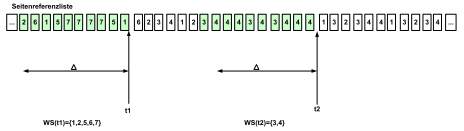
\includegraphics[width=1\columnwidth]{workingSet}
	\paragraph{Working Set Algorithmus} basiert auf dem Lokalitätsprinzip. \textbf{Annahmen}: R-Bit wird vom BS periodisch zurückgesetzt. R- und M-Bit durch die HW gesetzt. Seitentabelleneintrag mit Feld für \textbf{Zeitpunkt des letzten Zugriffs} und $\tau$ = Zeitintervall für Working Set\\ Bei einem \textit{Page Fault} $\rightarrow$ Seitentabelle durchsuchen (wird immer komplett durchlaufen, um Zugriffszeitpunkte zu aktualisieren). Falls \textbf{R=1}: Seite im Working Set $\rightarrow$ \textbf{Zugriffszeitpunkt auf aktuelle Zeit setzen}\\ Falls \textbf{R=0}: \textbf{Alter} der Seite $> \tau$ $\rightarrow$ Seite gehört nicht zum Working Set, also ersetzen\\ \textbf{Alter} $\leq \tau$ Älteste Seite merken. \textbf{Am Ende}: Älteste Seite ersetzen (mind. einmal war R=0 aber immer Alter $\leq \tau$) oder irgendeine, möglichst unveränderte Seite ersetzen (alle R=1)
	\paragraph{WSClock Algorithmus} Effizientere Implementierung, zyklisch verkettete Liste\\
	Bei \textit{Page Fault} starte bei Seite auf die der "Uhrzeiger" zeigt. Falls \textbf{R=1}, Seite wird benutzt $\rightarrow$ kein guter Kandidat, also setze R=0 und rücke zur nächsten Seite vor \\
	Falls \textbf{R=0} und \textbf{Alter $>\tau$} und \textbf{M=0} $\rightarrow$ Seite nicht überschreiben, Falls \textbf{R=0} und \textbf{Alter $>\tau$} und \textbf{M=1} Seite auf Festplatte schreiben und Zeiger vorrücken.
	\subsection{Speicherbelegung und Vergabe}
	\subsubsection{Speicherbelegungsstrategien}
	\paragraph{Speicherbelegungstabellen} Verwaltet die Belegung des Hauptspeichers
	\paragraph{Bitmap} Bits(0 = frei, 1 = belegt) werden einem Rahmen zugeordnet. Nebeneinander liegende Nullen deuten einen freien Hauptspeicherbereich an
	\subsubsection{Vergabestrategien}
	\paragraph{Sequentielle Suche} First-Fit: erster geeigneter Bereich wird vergeben
	\paragraph{Optimale Suche} Best-Fit: passender Bereich, um Fragmentierung zu vermeide, wird vergeben
	\paragraph{Buddy Technik} Stetige Halbierung des Speichers $\rightarrow$ Such nach dem kleinsten Bereich. Bereiche immer in $2^n$ aufteilen. Bei Hauptspeicherfreigabe werden Rahmen wieder zusammengefasst, die vorher getrennt wurden
	\subsection{Entladen (Cleaning)}
	Legt den Zeitpunkt fest, wann eine modifizierte Seite auf die Paging-Area geschrieben wird
	\paragraph{Demanding-Cleaning} Bei Bedarf! Seite lange im Hauptspeicher, aber Verzögerung bei Seitenwechsel
	\paragraph{Precleaning} Präventives Zurückschreiben, wenn Zeit ist! Frames in der Regel verfügbar
	\paragraph{Page-Buffering} Listen verwalten! Modified List: Zwischenpuffer, Unmodified List: Für Entladen freigeben
	\subsubsection{Lokale vs Globale Seitenersetzung}
	\paragraph{Lokale Strategie} Jeder Prozess hat eine feste Anzahl an Seitenrahmen. Beim \textit{Working Set} Algorithmus sinnvoll
	\paragraph{Globale Strategie} Meist besser: \textit{FIF}, \textit{LRU}, ...; Prozess entscheidet dynamisch, wie viel Speicher dem Prozess zugeteilt wird
	\section{Dateien \& Geräte}
	\subsection{Dateien und Verzeichnisse}
	persistente Speicherung von Informationen - von mehreren Prozessen gleichzeitig zugreifbar sein. \textit{Dateien} = abstrakter Mechanismus zur Speicherung und zum Wiederauffinden von Informationen
	\paragraph{Pseudodateien} z.B. Liste der defekten Blöcke eines Datenträgers
	\paragraph{Verzeichnisse} Verwaltung der Struktur des Dateisystems
	\paragraph{Metadaten} Informationen über die Datei selbst
	\subsubsection{Dateizugriff}
	\paragraph{Sequentieller Zugriff} Bytes werden nacheinander gelesen. Vor- und Zurückspringen nicht möglich
	\paragraph{Wahlfreier Zugriff} Bytes können in beliebiger Reihenfolge gelesen werden (Datenbanksysteme)
	\paragraph{Master Boot Record (MBR)} Ist auf Sektor 0, dient zum Booten des Rechnersystems. Enthält die \textit{Partitionstabelle}
	\paragraph{Partition Table} Liegt am Ende der MBR. Festplatte kann in mehrere Partitionen eingeteilt werden
	\paragraph{Bootblock} Wird beim Hochfahren gelesen und ausgeführt
	\paragraph{Superblock} Enthält Verwaltungsinformationen zum Dateisystem
	\paragraph{Free Blocks} Gibt die freien Blöcke des Dateisystems an
	\paragraph{Rootverzeichnis} Enthält den Inhalt des Dateisystems
	\paragraph{I-Nodes} sind Einträge im Inhaltsverzeichnis des Dateisystems
	\subsubsection{Implementierung von Dateien}
	Belegung durch verkettete Liste $\rightarrow$ Sequentieller Zugriff unkompliziert $\rightarrow$ Wahlfreier Zugriff extrem langsam. Verkettete Liste mit Tabelle im Arbeitsspeicher $\rightarrow$ \textit{File Allocation Table} (FAT)
	\subsubsection{File Allocation Table (FAT)}
	Speichert Datei als verkettete Liste von Plattenblöcken, hält die Information über Verkettung der Blöcke im Hauptspeicher. Vorteil: Wahlfreier Zugriff schneller, Verfolgen der Kette passiert im RAM. Nachteil: nicht praktikabel bei großen Festplatten
	\subsubsection{Implementierung von Verzeichnissen}
	\paragraph{Verzeichniseintrag} Enthält Informationen zum Auffinden der zugehörigen Plattenblöcke (Nr. des 1. Blocks $\vert$ Nr. des I-Nodes). Üblicherweise nicht sortiert. Dateiattribute können im Verzeichniseintrag gespeichert werden. Dateiattribute können im I-Node gespeichert werden (nur Verweis auf I-Node)
	\paragraph{Hard Link} Verzeichniseinträge verweisen auf den selben I-Node
	\paragraph{Symbolischer Link} Spezielle Datei vom Typ \textit{LINK}, welcher Pfad zur verlinkten Datei enthält\\
	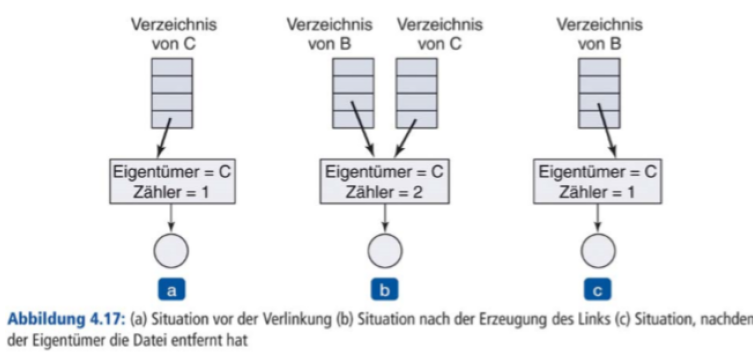
\includegraphics[width=0.8\columnwidth]{link}
	\subsubsection{Virtuelle Dateisysteme}
	\paragraph{Beispiele:} NTFS, ext, FATx für Festplatten - CD/DVD Dateisysteme - NFS (Network File System)\\\\
	Systemaufrufe (open, read, etc) gehen an die obere Schnittstelle des VFS - konkretes Dateisystem muss die untere Schnittstelle implementieren
	\subsubsection{Dateisystem Verwaltung}
	\paragraph{Datenrate vs. Platteneffizienz} Je mehr Daten mit einem einzigen Plattenzugriff geholt werden können, desto besser $\rightarrow$ Datenrate steigt mit der Blockgröße
	\subsubsection{Freie Blöcke verwalten}
	\paragraph{Verkettete Liste} 1KB-Block kann bis zu 255 Blocknummern (a 32 Bit) aufnehmen
	\paragraph{Bitmap} 1 Bit pro Block (0 = frei $\vert$ 1 = belegt)
	\subsubsection{Konsistenz}
	2 Tabellen mit Zählern für jeden Block. Tabelle 1 zählt, wie oft jeder Block in einer Datei vorkommt. Tabelle 2 zählt, wie oft jeder Block in der Freibereichsliste vorkommt. Jeder Block sollte genau einmal in Tabelle 1 oder in Tabelle 2 auftauchen\\
	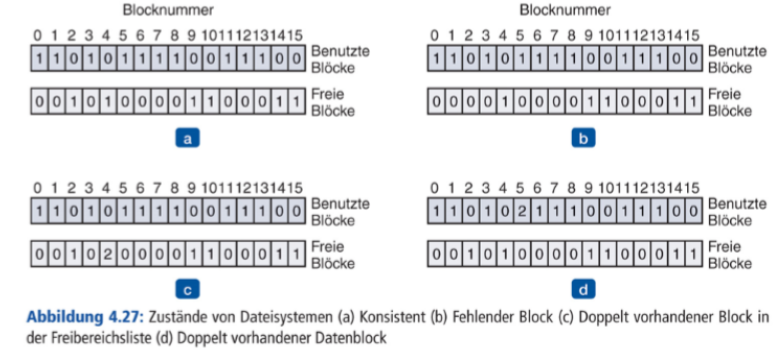
\includegraphics[width=0.95\columnwidth]{konsistenz}
	\paragraph{Gleicher Block} Lösung: in Freibereichsliste einfügen/löschen
	\paragraph{Doppelt vorhandener Block in Tabelle 2 (freie Blöcke)} nicht möglich, wenn freie Blöcke in einer Bitmap verwaltet werden $\rightarrow$ Freibereichsliste korrigieren
	\paragraph{Doppelt vorhandener Block in Tabelle 1 (benutzte Blöcke)} falls Datei gelöscht $\rightarrow$ Block sowohl benutzt als auch frei. Lösung: Block kopieren und Kopie einer der beiden Dateien zuweisen oder Benutzer informieren das Datei defekt ist
	\paragraph{Prüfung auf Dateiebene} hard Links $\rightarrow$ zählen wie oft eine Datei in Verzeichnissen auftaucht - Ergebnis mit Link-Zähler im I-Node der Datei vergleichen. \textbf{Link-Zähler zu hoch}: Nach dem Löschen der Datei in allen Verzeichnissen, wäre der Link-Zähler immer noch > 0 $\rightarrow$ \textbf{Lösung}: Link-Zähler korrigieren - \textbf{Link-Zähler zu klein}: Datei wird im Verzeichnis gelöscht $\rightarrow$ Link-Zähler = 0 $\rightarrow$ I-Node und die Blöcke werden freigegeben, obwohl sie benutzt werden - \textbf{Lösung}: Link-Zähler korrigieren
	\paragraph{Konsistenz - Journaling} \textbf{- Dateisysteme}
	\paragraph{Beispiel: Löschen einer Datei} Löschen einer Datei aus dem Verzeichnis - Freigeben des I-Node in den Pool der freien I-Nodes - Freigeben der Plattenblöcke in den Pool der freien Blöcke
	\paragraph{Zugehöriger Log-Eintrag} Listet die anstehenden Aktionen auf. \textit{Log-Eintrag} wird auf die Festplatte geschrieben - die Aktionen werden ausgeführt - Log-Eintrag wird gelöscht
	\subsubsection{Performanz}
	\paragraph{Caching} Block-Cache $\vert$ Puffer-Cache\\
	Menge von Blöcken im Speicher - Zugriff auf einen Block. Es wird geprüft ob er schon im Cache liegt. Falls nicht $\rightarrow$ wird in den Cache geladen - Suche mit Hashfunktion. \textbf{Problem}: Blöcke sollten nicht zu lange verändert im Cache liegen - selten wird mehrmals innerhalb einer kurzen Zeitspanne zugegriffen. \textbf{LRU-Schema anpassen}: Wenn Block bald wieder gebraucht wird $\rightarrow$ hinten in die LRU-Liste einfügen - wenn Block wichtig für die Konsistenz des Dateisystems $\rightarrow$ sofort auf die Platte schreiben
	\paragraph{UNIX/Linux - sync Systemaufruf} Bewirkt, dass alle Blöcke sofort auf die Festplatte geschrieben werden (dauert ca. 30s)
	\paragraph{Write-Through-Cache} Sobald Block verändert wird $\rightarrow$ sofort auf Festplatte schreiben (sicher, aber langsam)
	\paragraph{Bewegungen des Plattenarms reduzieren} Blöcke, auf die der Reihe nach zugegriffen werden $\rightarrow$ sollten nahe beieinander auf der Festplatte liegen. \textit{Bitmap} $\rightarrow$ zusammenhängende Blöcke können leicht gefunden werden. Alle I-Nodes liegen am Rand der Festplatte $\rightarrow$ durchschnittliche Entfernung I-Node und dem ersten Block der Datei = die Hälfte des Zylinderdurchmessers der Festplatte. \textbf{Besser}: I-Nodes in der Mitte platzieren $\vert$ Platte in Zylindergruppen einteilen
	\paragraph{Festplattenspeicher defragmentieren} Fragmentierung nimmt mit dem 'Vollsein' der Festplatte zu - Zusammengehörige Blöcke sind dann auf der Platte verteilt $\rightarrow$ Festplatte regelmäßig defragmentieren (Gilt nicht für SSD Festplatten $\rightarrow$ \textit{Wear out})
	\subsubsection{Dateisysteme}
	\paragraph{CD-ROM} Einfach strukturiert $\rightarrow$ Medium kann nur einmal beschrieben werden - keine Verwaltung der freien Blöcke nötig. \textbf{CD-R} $\rightarrow$ Dateien werden nie überschrieben, sondern am Ende der CD-R angehängt
	\paragraph{MS-DOS (FAT32, vFAT)} USB-Sticks, Digitalkameras, MP3-Player usw. $\rightarrow$ benutzt Datei-Allokationstabelle \textit{FAT}\\
	\textbf{Beispiel}: FAT-12 mit 512-Byte-Blöcken $\rightarrow$ $12 \cdot 512 Byte = 2MiB$ Partitionsgröße. FAT mit 4096 Einträgen a 2 Byte $\rightarrow$ 8KiB Hauptspeicher
	\paragraph{UNIX V7} Jeder I-Node (2 Byte für die I-Node Nummer $\rightarrow$ max. 65536 Dateien) hat eine feste Position auf der Festplatte
	\paragraph{Linux} \textit{Small is beautiful} $\rightarrow$ einfache Mechanismen und wenige Systemaufrufe (Verzeichnisbaum, Links, Virtuelles Filesystem / mounting)
	\paragraph{Prozess - Dateisystem proc} Enthält Informationen zum System und zu den laufenden Prozesse. Enthält \textit{Pseudodateien} (existieren nicht wirklich auf der Festplatte) - für jeden laufenden Prozess existiert ein Verzeichnis. Beim \textbf{Lesen}: System ermittelt Informationen durch Systemaufrufe. Beim \textbf{Schreiben}: Änderung der Systemparameter
	\paragraph{ext2 - Dateisystem} Partition in Gruppen von Blöcken aufgeteilt. I-Nodes und zugehörige Datenblöcke in der selben Gruppe am besten nah beieinander auf der Festplatte halten. Blöcke werden im Voraus für eine Datei reserviert - Verzeichniseinträge nicht sortiert - System speichert die kürzlich benutzten Verzeichnisse im Cache
	\paragraph{Superblock} Informationen über das Dateisystem $\rightarrow$ Layout, Anzahl I-Nodes, Anzahl Festplattenblöcke, etc.
	\paragraph{Gruppendeskriptor} Position der \textit{Bitmaps}, Anzahl freier Blöcke und I-Nodes, Anzahl der Verzeichnisse in der Gruppe
	\paragraph{Bitmaps} Verwaltung der freien I-Nodes und Blöcke. Jede Bitmap ist so groß wie ein Block
	\paragraph{Network File System (NFS)} Clients und Server nutzen Dateisystem gemeinsam. NFS-Server exportiert ein oder mehrere Verzeichnisse für den Zugriff von entfernten Clients - Jeder Rechner kann Client und Server sein
	\paragraph{NT Filesystem (NTFS)} Dateikompression, Journaling, alternative Datenströme, 64 Bit-Adressen für Blöcke $\rightarrow$ wichtigste Datenstruktur: \textit{Masterdateitabelle (MFT)} 
	\paragraph{Master File Table (MFT)} Einträge sind ein 1KiB groß und beschreiben Datein oder Verzeichnisse. Freie MFT werden mit \textit{Bitmap} verwaltet. MFT ist eine Datei - Datenblöcke einer Datei werden in Form von Serien aufeinanderfolgender Blöcke gespeichert $\rightarrow$ Je mehr Fragmentierung, desto mehr MFT-Datensätze werden benötigt
	\paragraph{Datenkompression} Gruppen von 16 logischen Blöcken werden komprimiert gespeichert, wenn sie dann nur noch 15 oder weniger Blöcke belegen $\rightarrow$ Zugriff schwieriger, da evtl. zuerst dekomprimiert werden muss
	\paragraph{Alternative Datenströme} (Zusätzliche Datenattribute) Wird benutzt für: Schadcode oder getrennte Audio- und Videostreams in einer Datei
	\subsection{Geräteverwaltung}
	\subsubsection{Grundlagen}
	Verwaltung von externen Geräten - durch Abstraktion $\rightarrow$ leicht zu bedienende Schnittstelle. \textbf{Aufgaben}: Kommandos an Geräte senden, Daten empfangen und weiterleiten, Interrupts behandeln, Fehlerbehandlung
	\paragraph{Geräte-Datei} Eine spezielle (\textit{Pseudo-}) Datei unter Linux, die ein Gerät repräsentiert (z.B. Drucker). Durch Lese-/Schreiboperationen auf die Datei wird auf das entsprechende Gerät zugegriffen
	\paragraph{Blockorientierte Geräte} Speichern Daten in Blöcken fester Größe, welche einzeln adressierbar sind
	\paragraph{Zeichenorientierte Geräte} Erzeugen bzw. lesen Zeichenströme. Nicht adressierbar
	\paragraph{Controller} Gerät besteht aus 2 Komponenten. Mechanische und elektronische (Controller/Steueinheit) - ein Controller kann auch mehrere Geräte verwalten. \textbf{Aufgaben}: Seriellen Bit-Stream in Byte-Blöcke konvertieren, Fehlerkorrektur, Daten in den Arbeitsspeicher kopieren
	\paragraph{Controller-Schnittstelle} Schnittstelle welche für was jedes Gerät anders ist. Controller besitzt eine Menge von Kontrollregistern zur Ansteuerung. \textbf{Schreiben} in ein Register $\rightarrow$ Befehle erteilen, Aktionen auslösen. \textbf{Lesen} eines Registers $\rightarrow$ Statusinformationen. \textbf{Datenpuffer}, die lesen/geschrieben werden können. \textbf{Zugriff auf die Kontrollregister}: Der Zugriff kann auf zwei Arten erfolgen. Register liegen in einem eigenen, getrennten Adressraum\\
	Register werden in den Arbeitsspeicher eingeblendet $\rightarrow$ \textbf{Memory-Mapped I/O}
	\paragraph{Memory-Mapped I/O} Zugriff auf getrennten Bereich erfolgt über Assembler-Befehle. Die Kontrollregister liegen am Rand des Adressraumes. Jedes Gerät hat eine eindeutige Adresse
	\paragraph{Memory-Mapped I/O - Vorteile} Kann in C/C++ programmiert werden, einfach Zugriffskontrolle
	\paragraph{Memory-Mapped I/O - Nachteile} Caching muss für den Seitenrahmen ausgeschaltet werden - bei jedem Speicherzugriff muss unterschieden werden, ob es sich um ein Kontrollregister handelt oder nicht
	\paragraph{Direct Memory Access(DMA)} Ablauf ohne Direct Memory Access $\rightarrow$ Lesen von einer Festplatte. Plattencontroller liest einen Block byteweise von der Festplatte - speichert Block in seinen internen Puffer - Festplattencontroller berechnet Prüfsumme und führt ggf. Fehlerkorrektur durch. Plattencontroller erzeugt einen Interrupt. Betriebssystem kopiert den Pufferinhalt byteweise in den Arbeitsspeicher $\rightarrow$ viel Aufwand für das Betriebssystem\\
	Der DMA-Controller lohnt sich nur, wenn der Prozessor tatsächlich etwas anderes zu tun hat
	\subsubsection{Ein-/Ausgabe Software, Treiber}
	\paragraph{Geräteunabhängigkeit} Programme können Geräte ansprechen ohne es genau zu kennen
	\paragraph{Benennungsschema} Name unabhängig von der Art des Gerätes
	\paragraph{Fehlerbehandlung} Sollte nah an der Hardware stattfinden
	\paragraph{Synchronisation} Synchron oder Asynchron
	\paragraph{Puffern} Daten können meist nicht direkt im Speicherziel abgelegt werden
	\paragraph{Nutzung} Exklusiv oder Gemeinsam
	\paragraph{Programmierte Ein-/Ausgabe} Das Betriebssystem übernimmt die komplette Übertragung zum Gerät $\rightarrow$ Prozessor ist während der gesamten Ein-/Ausgabe belegt\\
	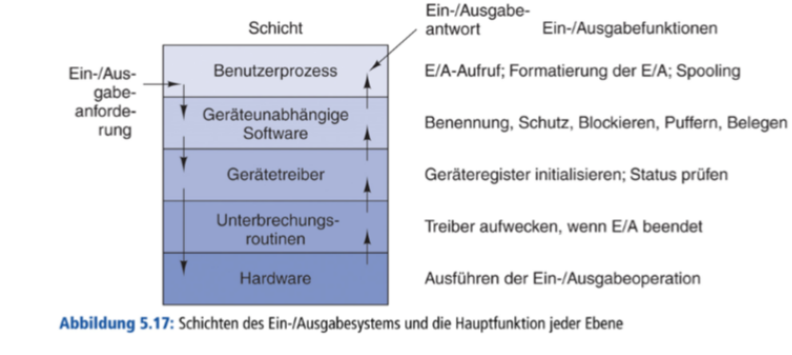
\includegraphics[width=0.95\columnwidth]{einausgabe}
	\paragraph{Treiber} Ansteuern des Controllers ist die Aufgabe des Treibers (gerätespezifischer Programmteil). Meist durch den Gerätehersteller in eigenen Modulen realisiert. \textbf{Aufgaben}: Initialisierung und Bekanntgabe des Gerätes, Datenübertragung von und zu einem Gerät, Logisches Programmiermodell auf gerätespezifische Anforderungen übersetzen, Pufferung vn Daten, Interruptverarbeitung, Koordination der nebenläufigen Zugriffe. Treiber sind im Betriebssystem integriert $\rightarrow$ Treiber kann das gesamte System zum Absturz bringen
	\paragraph{Integration von} \textbf{Treibern}
	\paragraph{Statisch} Beim Compilieren des Kerns werden alle Treiber eingebunden
	\paragraph{Dynamisch} Treiber werden ins laufende System nachgeladen
	\paragraph{Schnittstellen für Treiber} Das Betriebssystem definert eine Standardschnittstelle und - Architektur für die Installation von Treibern. Standardschnittstelle für blockorientierte Gerätetreiber. Standardschnittstelle für zeichenorientierte Gerätetreiber
	\section{Betriebssystemvirtualisierung}
	\subsection{Grundlagen, Begriffe}
	\paragraph{Definition Virtualisierung} Nachbildung eines Hard- oder Software Objekts durch ein ähnliches Objekt mit Hilfe einer Softwareschicht
	\paragraph{Virtuelle Maschine (VM)} Nachbildung eines kompletten Rechners durch einen ähnlichen oder ganz anderen Rechner (Softwareschicht: Hypervisor oder Virtual Machine Monitor)
	\paragraph{Vorteile von VMs} Mehrere Betriebssysteme auf dem Rechner - bessere Nutzung leistungsfähiger Hardware durch mehrere virtuelle Server auf nur einem realen Rechner - einfaches Kopieren eiber VM
	\paragraph{Nachteile von VMs} VMs müssen sich die real vorhandenen Ressourcen auf einem Rechner teilen - Ausfall des realen Rechners $\rightarrow$ Ausfall aller VMs. Virtualisierung (VMM) benötigt selbst Ressourcen
	\paragraph{Emulation} Jeder einzelne Maschinenbefehl des nachgebildeten Rechners wird durch Software ausgeführt $\rightarrow$ langsam, Geschwindigkeitsverlust Faktor 5 bis 10
	\paragraph{Virtualisierung} Die meisten Maschinenbefehle des nachgebildeten Rechners werden auf dem nachgebildeten Rechner nativ, also ohne Software-Eingriff direkt durch dessen Hardware ausgeführt
	\subsubsection{Virtual Machine Monitor (VMM)}
	\paragraph{Aufgabe} Bereitstellen von isolierten Ablaufumgebungen in Form von Duplikaten der realen Hardware
	\paragraph{Implementierung} VMM fängt an bestimmte Maschinenbefehle ab und ersetzt diese durch andere, VM-spezifische Aktionen
	\subsection{Voraussetzungen}
	\paragraph{Mindestvoraussetzung} Unterscheidung zwichen Kernel- und Anwendungsmodus des Prozessors. Vorhandensein einer MMU zur Abschottung von Adressräumen der VMs
	\paragraph{Problem mit den sensitiven Befehlen} Es gibt privilegierte und nicht privilegierte Befehle im Befehlssatz von Prozessoren. Privilegierte Befehle läsen Sprünge ins Betriebssystem aus. Sensitive Befehle sind zustandsverändernd und dürfen nur im Kernelmodus ausgeführt werden
	\paragraph{Virtualisierbarkeit nach Popek und Goldberg Theorem} Prozess ist virtualisierbar, wenn alle privilegierten Maschinenbefehle eine Unterbrechung erzeugen, wenn die in einem unprivilegierten Prozessormodus ausgeführt werden. Alle sensitiven Befehle sind auch privilegierte Befehle
	\paragraph{Kritische Befehle} Lösung: Dynamische Übersetzung kritischer Befehle zur Laufzeit durch direkte Aufrufe an den VMM. Code des Gast-Betriebssystems vor Abarbeitung in einen Puffer laden. Nach den kritischen Befehlen durchsuchen $\rightarrow$ durch direkte Aufrufe an den VMM ersetzen
	\subsubsection{Arten der Virtualisierung}
	\paragraph{(VMM=) Typ-1-Hypervisor} Direkt über Hardware als kleines Minibetriebssystem - benötigt HW-Unterstützung für Virtualisierung im Prozessor. VMM \textbf{muss} alle Treiber zur Verfügung stellen
	\paragraph{Typ-2-Hypervisor} VMM läuft als Prozess unter einem Wirtsbetriebssystem $\rightarrow$ kann die Treiber des Wirtbetriebssystems mitnutzen - Das Wirtsbetriebssystem ist auch direkt zugänglich
	\paragraph{Arten der Virtualisierung} Paravirtulaisierung mit Modifikationen des Gast-Betriebssystems
	\paragraph{Übersetzungszeit} Ersetzung kritischer Maschinenbefehle im Gast-Betriebssystem durhc direkte Aufrufe an den VMM
	\paragraph{Vorteil} Unabhängigkeit von den oben genannten Voraussetzungen, Durchsatzsteigerung
	\paragraph{Nachteil} Gast-Betriebssystem muss im Quellcode zugänglich sein
	\subsubsection{Speicher- und Gerätevirtualisierung}
	\paragraph{Schattentabellen} Für jede VM eine Schattentabelle - übersetzt gastphysische Adresse in physische Adresse
	\paragraph{Geräteemulation} VMM betreibt das Gerät via eigenem Treiber oder Treiber des Wirtsbetriebssystem. VMM bietet dem Gastbetriebssystem eine Schnittstelle zu einem Standard-Gerät. Gastbetriebssystem kann seine eigenen Treiber verwenden
	\paragraph{Direktzuweisung eines Gerätes} Gerät wird einem Gastbetriebssystem exklusiv zugewiesen. Das Gastbetriebssystem interagiert via seinem eigenen Treiber direkt, also unter Umgebung des VMM, mit dem Gerät
	\section{Storage Systems}
	\subsection{RAID Systeme}
	RAID: \textit{Redundant Array of Inexpensive Disks} multiple Plattenspeicher - mehrere kleine Platten werden als eine große virtuelle Platte verwaltet. Für das Betriebssystem transparent
	\paragraph{RAID - 0} Stripes werden über mehrere Platten eines Arrays verteilt. Verteilung übernimmt das Betriebssystem oder eigener RAID-Controller $\rightarrow$ hoher I/O-Durchsatz, aber nicht ausfallsicher
	\paragraph{RAID - 1} wie RAID - 0, aber mit Redundanz. \textbf{Schreiben}: Jedes Stripe wird doppelt geschrieben. \textbf{Lesen}: Eine der beiden Kopien kann genutzt werden
	\paragraph{RAIN - 2} Platten laufen synchron - jedes Byte wird in 2 Halbbytes aufgeteilt. Zu jedem Halbbyte wird ein Hamming-Code hinzugefügt
	\paragraph{RAID - 3} 1-Bit-Fehlerkorrektur $\rightarrow$ Bei Ausfall einer Platte kann das fehlende Bit wiederhergestellt werden
	\paragraph{RAID - 4, RAID - 5} Stripe-Parität: XOR-Operation auf alle Stripes $\rightarrow$ bei Ausfall kann die fehlende Platte wiederhergestellt werden
	\paragraph{NAS - Network Attached Storage} Massenspeichereinheiten, die an ein lokales Netzwerk (LAN) angeschlossen sind
	\paragraph{SAN - Storage Area Network} Eigenes Netzwerk zwischen Servern und den Speicherressourcen. Speicher kann virtuell wie eine einzige Festplatte behandelt werden
	\end{multicols*}
\end{document}